% !Mode:: "Tex:UTF-8"



\documentclass[10pt,a4paper]{article}\usepackage[]{graphicx}\usepackage[]{color}
%% maxwidth is the original width if it is less than linewidth
%% otherwise use linewidth (to make sure the graphics do not exceed the margin)
\makeatletter
\def\maxwidth{ %
  \ifdim\Gin@nat@width>\linewidth
    \linewidth
  \else
    \Gin@nat@width
  \fi
}
\makeatother

\definecolor{fgcolor}{rgb}{0.345, 0.345, 0.345}
\newcommand{\hlnum}[1]{\textcolor[rgb]{0.686,0.059,0.569}{#1}}%
\newcommand{\hlstr}[1]{\textcolor[rgb]{0.192,0.494,0.8}{#1}}%
\newcommand{\hlcom}[1]{\textcolor[rgb]{0.678,0.584,0.686}{\textit{#1}}}%
\newcommand{\hlopt}[1]{\textcolor[rgb]{0,0,0}{#1}}%
\newcommand{\hlstd}[1]{\textcolor[rgb]{0.345,0.345,0.345}{#1}}%
\newcommand{\hlkwa}[1]{\textcolor[rgb]{0.161,0.373,0.58}{\textbf{#1}}}%
\newcommand{\hlkwb}[1]{\textcolor[rgb]{0.69,0.353,0.396}{#1}}%
\newcommand{\hlkwc}[1]{\textcolor[rgb]{0.333,0.667,0.333}{#1}}%
\newcommand{\hlkwd}[1]{\textcolor[rgb]{0.737,0.353,0.396}{\textbf{#1}}}%
\let\hlipl\hlkwb

\usepackage{framed}
\makeatletter
\newenvironment{kframe}{%
 \def\at@end@of@kframe{}%
 \ifinner\ifhmode%
  \def\at@end@of@kframe{\end{minipage}}%
  \begin{minipage}{\columnwidth}%
 \fi\fi%
 \def\FrameCommand##1{\hskip\@totalleftmargin \hskip-\fboxsep
 \colorbox{shadecolor}{##1}\hskip-\fboxsep
     % There is no \\@totalrightmargin, so:
     \hskip-\linewidth \hskip-\@totalleftmargin \hskip\columnwidth}%
 \MakeFramed {\advance\hsize-\width
   \@totalleftmargin\z@ \linewidth\hsize
   \@setminipage}}%
 {\par\unskip\endMakeFramed%
 \at@end@of@kframe}
\makeatother

\definecolor{shadecolor}{rgb}{.97, .97, .97}
\definecolor{messagecolor}{rgb}{0, 0, 0}
\definecolor{warningcolor}{rgb}{1, 0, 1}
\definecolor{errorcolor}{rgb}{1, 0, 0}
\newenvironment{knitrout}{}{} % an empty environment to be redefined in TeX

\usepackage{alltt}
\usepackage{etoolbox}
\newtoggle{color}
%\togglefalse{color}
\toggletrue{color}

\usepackage{makeidx}
\newcommand{\idioma}{spanish}
\newcommand{\opcionesIdioma}{,es-nodecimaldot,es-tabla}
% !Mode:: "Tex:UTF-8"
%%%%%%%%%%%%%%%%%%%%%Carga de Packages
%%poner \newcommand{\idioma}{spanish} o \newcommand{\idioma}{english} en el documento
\usepackage{pdfsync}
\usepackage{srcltx}
\usepackage[\idioma\opcionesIdioma]{babel}
\usepackage[utf8x]{inputenc}
\usepackage[T1]{fontenc}
\usepackage{graphicx}
\graphicspath{{/users/fernando/figuras/}{./}{./figuras/}{/fernando/figuras/}{/fernando/figuras/jpg/}}
\usepackage{multicol}
\usepackage{epsfig}
%\usepackage{oberdiek}
\usepackage{listingsutf8}
\lstset{inputencoding=utf8/latin1}
%\lstset{extendedchars=true}
\lstset{ %
  language=R,                     % the language of the code
  basicstyle=\ttfamily\small,       % the size of the fonts that are used for the code
  numbers=left,                   % where to put the line-numbers
  numberstyle=\tiny\color{gray},  % the style that is used for the line-numbers
  stepnumber=1,                   % the step between two line-numbers. If it's 1, each line
                                  % will be numbered
  numbersep=5pt,                  % how far the line-numbers are from the code
  backgroundcolor=\color{white},  % choose the background color. You must add \usepackage{color}
  showspaces=false,               % show spaces adding particular underscores
  showstringspaces=false,         % underline spaces within strings
  showtabs=false,                 % show tabs within strings adding particular underscores
  frame=single,                   % adds a frame around the code
  rulecolor=\color{black},        % if not set, the frame-color may be changed on line-breaks within not-black text (e.g. commens (green here))
  tabsize=2,                      % sets default tabsize to 2 spaces
  %captionpos=,                   % sets the caption-position to bottom
  breaklines=true,                % sets automatic line breaking
  breakatwhitespace=false,        % sets if automatic breaks should only happen at whitespace
  %title=\lstname,                 % show the filename of files included with \lstinputlisting;
                                  % also try caption instead of title
  keywordstyle=\color{black},      % keyword style
  commentstyle=\color{Brown},   % comment style
  stringstyle=\color{black},      % string literal style
  escapeinside={\%*}{*)},         % if you want to add a comment within your code
  morekeywords={*,...},            % if you want to add more keywords to the set
  lineskip={-2.5pt} % single line spacing
}
%\usepackage{algorithm}
\usepackage{amsmath}
\usepackage{amsfonts}
\usepackage{amssymb}
\usepackage{amsthm}
\usepackage{fancybox}
\usepackage{fancyvrb}
\usepackage{rotating}
\usepackage{keystroke}
\usepackage{array}
\input{xy}
\xyoption{all}
%\usepackage[dvipsnames,usenames]{color}
\usepackage[usenames,dvipsnames,svgnames,table]{xcolor}
\usepackage{colortbl}
\usepackage{comment}
\excludecomment{spanish}
\excludecomment{english}
\includecomment{\idioma}

%\usepackage{noweb}
%\usepackage{clrscode}
\usepackage{eurosym}
\usepackage{wasysym}
\usepackage{multirow}
%\usepackage{margins}
\usepackage{lscape}
\usepackage{longtable}
\usepackage[normalem]{ulem}
\usepackage{xr-hyper}

%%NUEVO
\newcolumntype{C}{{\centering\arraybackslash}m{20mm}}
\newcommand{\centercell}[1]{\multicolumn{1}{c}{#1}}
\newcommand{\colHead}[1]{\centercell{\bfseries#1}}

\excludecomment{ocultar}


% Matriz (par‚ntesis)
\def\matr#1#2{\left(\begin{array}{#1}#2\end{array}\right)}
% Determinante (barras)
\def\deter#1#2{\left|\begin{array}{#1}#2\end{array}\right|}
% Sistema de ecuaciones. (llave a la izda.)
\def\seq#1#2{\left\{\begin{array}{#1}#2\end{array}\right.}
% Ecuaci\'on de varias lineas (sin llave a la izda.)
\def\evl#1#2{\begin{array}{#1}#2\end{array}}

%%%%%%%%%%%%%%%%%%%%%%%%%%%%%%%%%%%%%%%%%%%%%%
%%%%%%%%%%%%%%%%%%%%%%%%%%%%%%%%%%%%%%%%%%%%%%
%%%%%%%%%%%%%%%%% M\'{a}rgenes %%%%%%%%%%%%%%%%
%
%
%\parindent=0mm
%
%\textwidth=160mm
%\textheight=220mm
%\hoffset=-20mm
%\voffset=-15mm
%\parskip=0mm
\marginparsep=3mm
\marginparwidth=25mm
%
%%%%%%%%%%%%%%%%%%%%%%%%%%%% Contadores para listas de problemas
%\newcommand{\adc}{\addtocounter{enumi}{1}}
\newcommand{\adc}{\stepcounter{enumi}}
\newcommand{\adci}{\stepcounter{enumii}}
\newcommand{\xadc}{\addtocounter{xcounter}{1}}
\newcommand{\be}{\begin{enumerate}}
\newcommand{\ee}{\end{enumerate}}
\newcommand{\bi}{\begin{itemize}}
\newcommand{\ei}{\end{itemize}}
\newcounter{xcounter}


\newcommand{\nin}{{\noindent}}

%\newcounter{prob}{}
%\def\pr{\addtocounter{prob}{1}(\theprob)\ }
%\def\pr2{\addtocounter{prob}{2}(\theprob)\ }

%%%%%%%%%%%%%%%%%%%%%%%%%%%Fin de demostraciones, ejemplos, etc.
\newcommand{\fin}{$\square$}
%%%%%%%%%%%%%%%%%%%%%%%%%%Notaci\'{o}n matem\'{a}ticas generales
%\newcommand{\suc}[1]{\{#1_n\}}
%\newcommand{\sucn}[1]{\{#1_n\}_{n\in\mathbb{N}}}
%\newcommand{\ser}[1]{\sum #1_n}
%\newcommand{\sern}[1]{\sum_{n\geq 1} #1_n}
%\newcommand{\limn}{\lim_{n\rightarrow\infty}}
%\newcommand{\limnd}{\displaystyle\lim_{n\rightarrow\infty}}
%\newcommand{\mf}[1]{\mathbf{#1}}
%\newcommand{\mb}[1]{\mathbb{#1}}
%\newcommand{\D}[1]{\Dv_{\mf{#1}}}
%\newcommand{\bsigma}{\pmb{\sigma}}
%\newcommand{\bPhi}{\pmb{\Phi}}
%\newcommand{\vol}{\operatorname{vol}}
%\newcommand{\ldbr}{[\hspace{-1.5pt}[}
%\newcommand{\rdbr}{]\hspace{-1.5pt}]}
%\newcommand{\fpws}[2]{{#1}\ldbr{#2}\rdbr}
%\newcommand{\leftPui}{<\hspace{-3pt}<}
%\newcommand{\rightPui}{\hspace{-3pt}}
%\newcommand{\Pui}[2]{{#1}\hspace{-6pt}\leftPui{#2}\rightPui}
%\newcommand{\pdd}[2]{\dfrac{\partial{#1}}{\partial{#2}}}
%%%%%%%%%%Conjuntos de n\'{u}meros
\newcommand{\N}{\mathbb{N}} %conjunto de n\'{u}meros naturales
\newcommand{\Z}{\mathbb{Z}} %conjunto de n\'{u}meros enteros
\newcommand{\R}{\mathbb{R}} %conjunto de n\'{u}meros reales
\newcommand{\C}{\mathbb{C}} %conjunto de n\'{u}meros complejos
\newcommand{\Q}{\mathbb{Q}} %conjunto de n\'{u}meros racionales
\newcommand{\EP}{\mathbb{P}} %espacios proyectivos
\newcommand{\K}{\mathbb{K}} %cuerpo gen\'{e}rico
\newcommand{\A}{\mathbb{A}} %espacios afines

%%%%%%%%%%Estadistica
\newcommand{\MEAN}{\mathrm{E}}
\newcommand{\Var}{\mathrm{Var}}
\newcommand{\Cov}{\mathrm{Cov}}


%%%%%%%%%%Funciones
\def\arcsen{\operatorname{arcsen}}
\def\arctg{\operatorname{arctg}}
\def\argCosh{\operatorname{argCosh}}
\def\argSenh{\operatorname{argSenh}}
\def\argTgh{\operatorname{argTgh}}
\def\cosec{\operatorname{cosec}}
\def\Cosh{\operatorname{Cosh}}
\def\cotg{\operatorname{cotg}}
\def\Dv{\operatorname{D}}
\def\discrim{\operatorname{discrim}}
\def\dive{\operatorname{div}}
\def\dom{\operatorname{dom}}
\def\Ext{\operatorname{Ext}}
\def\Fr{\operatorname{Fr}}
\def\dder#1#2{\dfrac{d #1}{d #2} } %derivada en estilo display
\def\gr{\operatorname{gr}}
\def\grad{\operatorname{grad}}
\def\Imag{\operatorname{Im}}
\def\mcm{\operatorname{mcm}}
\def\rang{\operatorname{rang}}
\def\rot{\operatorname{rot}}
\def\sen{\operatorname{sen}}
\def\Senh{\operatorname{Senh}}
\def\sgn{\operatorname{sgn}}
\def\sig{\operatorname{sig}}
\def\tg{\operatorname{tg}}
\def\Tgh{\operatorname{Tgh}}
\def\E{\operatorname{E}}
\def\VAR{\operatorname{VAR}}
\newcommand{\margWeb}[2]{\noindent{#2}\marginpar[\hspace{-18mm}\link{#1}{WEB}]{\hspace*{-18mm}\link{#1}{WEB}}}

%%%%%%%%%%%%%%%%%%%%%%\'{A}lgebra conmutativa.
\def\multideg{\operatorname{multideg}} %multidegree of a polynomial
\def\LT{\operatorname{lt}} %leading term of a polynomial
\def\LC{\operatorname{lc}} %leading coefficient of a polynomial
\def\LM{\operatorname{lm}} %leading monomial of a polynomial
\def\Mexp{\mathbb{Z}^n_{\geq 0}} %set of multiexponents of monomials
\def\set#1{\left\{{#1}\right\}}
\newcommand{\vlist}[2]{\mbox{${#1}_{1},\ldots,{#1}_{#2}$}}
\def\deg{\operatorname{deg}} %grado de un polinomio
\def\cp{\operatorname{cp}} %coeficiente principal de un polinomio
\def\CP{\operatorname{cp}} %coeficiente principal de un polinomio
\def\set#1{\left\{{#1}\right\}} %llaves de conjunto
\newcommand{\V}{{\bf V}} %variedad de un conjunto de polinomios
\newcommand{\I}{{\bf I}} %ideal de un conjunto
\newcommand{\MCD}{\operatorname{mcd}} %m\'{a}ximo com\'{u}n divisor
\newcommand{\MCM}{\operatorname{mcm}} %m\'{\i}nimo com\'{u}n m\'{u}ltiplo
\newcommand{\LCM}{\operatorname{lcm}} %least common multiple
\newcommand{\GCD}{\operatorname{gcd}} %greatest common divisor
\newcommand{\Ker}{\operatorname{Ker}} %N\'{u}cleo
\newcommand{\IM}{\operatorname{IM}} %Imagen
\newcommand{\Rad}{\operatorname{Rad}} %radical de un ideal
\newcommand{\Jac}{\operatorname{Jac}} %radical de Jacobson de un anillo
\newcommand{\Ann}{\operatorname{Ann}} %anulador de un ideal
\newcommand{\Res}{\operatorname{Res}} %resultante de polinomios
\newcommand{\Mult}{\operatorname{mult}} %multiplicidad
\newcommand{\Gen}{\operatorname{Gen}} %g\'{e}nero
\newcommand{\Card}{\operatorname{Card}} %cardinal
\newcommand{\ord}{\operatorname{ord}} %orden
\newcommand{\prim}{\operatorname{prim}} %parte primitiva
\newcommand{\NP}{\operatorname{NP}} %NP idea
\newcommand{\cont}{\operatorname{cont}} %parte primitva
\newcommand{\pp}{\operatorname{pp}} %parte primitva
\newcommand{\PP}{\mathop{\mathrm{PP}}\nolimits}
\newcommand{\Int}{\operatorname{Int}}
\newcommand{\Ind}{\operatorname{index}}
\newcommand{\Lcoeff}{\operatorname{lc}} %leading coefficient of a polynomial
\newcommand{\Sqf}{\operatorname{Sqf}} %square free part of a polynomial

\def\pd#1#2{\frac{\partial #1}{\partial #2}} %derivada parcial
\def\mult{\text{mult}} %multiplicity
\def\Sing{\text{Sing}} %multiplicity
\def\Cl#1{\overline{#1}} %cierre topol\'{o}gico
\def\fobox#1{\begin{center}\fbox{$\displaystyle #1 $}\end{center}}

%\newcommand{\Ext}{\operatorname{Ext}}

%%%%%%%%%%%%%%%%%%%%%%%%
%% unpunto mayor que cdot, pero menor que bullet
\newcommand{\sbt}{\,\begin{picture}(-1,1)(-1,-3)\circle*{3}\end{picture}\ }

%%%%%%%%%%%%%%%%%%%%%%%%S\'{\i}mbolos rodeados de un c\'{\i}rculo
\def\circled#1{\xymatrix{*+[o][F]{#1}}}

%%%%%%%%%%%%%%%%%%%Geometr\'{\i}a
\newcommand{\CH}{{\cal CH}} %%cierre convexo

%%%%%%%%%%%%%%%%%%%%Tipos de letra especiales
%%Caligr\'{a}ficas
\newcommand{\cA}{{\cal A}}
\newcommand{\cB}{{\cal B}}
\newcommand{\cC}{{\cal C}}
\newcommand{\cD}{{\cal D}}
\newcommand{\cE}{{\cal E}}
\newcommand{\cF}{{\cal F}}
\newcommand{\cG}{{\cal G}}
\newcommand{\cH}{{\cal H}}
\newcommand{\cI}{{\cal I}}
\newcommand{\cJ}{{\cal J}}
\newcommand{\cK}{{\cal K}}
\newcommand{\cL}{{\cal L}}
\newcommand{\cM}{{\cal M}}
\newcommand{\cN}{{\cal N}}
\newcommand{\cO}{{\cal O}}
\newcommand{\cP}{{\cal P}}
\newcommand{\cQ}{{\cal Q}}
\newcommand{\cR}{{\cal R}}
\newcommand{\cS}{{\cal S}}
\newcommand{\cT}{{\cal T}}
\newcommand{\cU}{{\cal U}}
\newcommand{\cV}{{\cal V}}
\newcommand{\cW}{{\cal W}}
\newcommand{\cX}{{\cal X}}
\newcommand{\cY}{{\cal Y}}
\newcommand{\cZ}{{\cal Z}}

%%%%%%%%%%%%%%%%%%%%%%%%%%Notaci\'{o}n matem\'{a}ticas generales
\newcommand{\sucn}[1]{\{#1_n\}_{n\in\mathbb{N}}}
\newcommand{\ser}[1]{\sum #1_n}
\newcommand{\sern}[1]{\sum_{n\geq 1} #1_n}
\newcommand{\limn}{\lim_{n\rightarrow\infty}}
\newcommand{\mf}[1]{\mathbf{#1}}
\newcommand{\mb}[1]{\mathbb{#1}}
\newcommand{\D}[1]{\Dv_{\mf{#1}}}
\newcommand{\bsigma}{\pmb{\sigma}}
\newcommand{\bPhi}{\pmb{\Phi}}
\newcommand{\vol}{\operatorname{vol}}
\newcommand{\ldbr}{[\hspace{-1.5pt}[}
\newcommand{\rdbr}{]\hspace{-1.5pt}]}
\newcommand{\fpws}[2]{{#1}\ldbr{#2}\rdbr}
\newcommand{\leftPui}{<\hspace{-3pt}<}
\newcommand{\rightPui}{\hspace{-3pt}}
\newcommand{\Pui}[2]{{#1}\hspace{-6pt}\leftPui{#2}\rightPui}
\newcommand{\pdd}[2]{\dfrac{\partial{#1}}{\partial{#2}}}


%\newcounter{contEnlace}

%\newcommand{\pendiente}{\textcolor{purple}{PENDIENTE: }}
%\newcommand{\link}[2]{\textcolor{blue}{{\href{#1}{#2}}}}


\iftoggle{color}{%
  % color version
  \newcommand{\pendiente}{\textcolor{red}{PENDIENTE: }}
  \newcommand{\link}[2]{\textcolor{blue}{{\href{#1}{#2}}}}
  \newcommand{\fichero}[2]{\textattachfile{#1}{\textcolor{blue}{#2}}}
  \newcommand{\otrofichero}[2]{\textattachfile{./datos/#1}{\textcolor{blue}{#2}}}
}{%
  % b/w version
  \newcommand{\pendiente}{\textcolor{black}{\underline{PENDIENTE:} }}
  \newcommand{\link}[2]{\textcolor{black}{{\href{#1}{\underline{#2}}}}}
  \newcommand{\fichero}[2]{\textattachfile{#1}{\textcolor{black}{\underline{#2}}}}
  \newcommand{\otrofichero}[2]{\textattachfile{./datos/#1}{\textcolor{black}{\underline{#2}}}}
}



%{\textcolor{blue}{{\href{#1}{#2}}}}

%%%%%%%%%%%%%%%%%%COLORES

\DefineNamedColor{named}{Brown}{cmyk}{0,0.81,1,0.60}
\definecolor{Gris050}{gray}{0.50}
\definecolor{Gris025}{gray}{0.75}
\definecolor{Gris010}{gray}{0.90}


%%%%%%%%%%%%%%%%%%%%%Package Algorithms
%\begin{spanish}
%\renewcommand{\algorithmicrequire}{{precondici\'{o}n:}}
%\renewcommand{\algorithmicensure}{{postcondici\'{o}n:}}
%\renewcommand{\algorithmicend}{{fin}}
%\renewcommand{\algorithmicif}{{si}}
% \renewcommand{\algorithmicthen}{{entonces}}
% \renewcommand{\algorithmicelse}{{si no}}
% \renewcommand{\algorithmicelsif}{\algorithmicelse\ \algorithmicif}
% \renewcommand{\algorithmicendif}{\algorithmicend\ \algorithmicif}
% \renewcommand{\algorithmicfor}{{para}}
% \renewcommand{\algorithmicforall}{{para todo}}
% \renewcommand{\algorithmicdo}{{hacer}}
% \renewcommand{\algorithmicendfor}{\algorithmicend\ \algorithmicfor}
% \renewcommand{\algorithmicwhile}{{mientras}}
% \renewcommand{\algorithmicendwhile}{\algorithmicend\ \algorithmicwhile}
% \renewcommand{\algorithmicrepeat}{{repetir}}
% \renewcommand{\algorithmicuntil}{{hasta}}
% \end{spanish}

%%%%%%%%%%%%%%%%%%%%%%%%%%%%%%%%%%Package Amsthm
\begin{spanish}
%\theoremstyle{definition}% default
\theoremstyle{plain}
\newtheorem{thm}{Teorema}[section]
\newtheorem{teo}{Teorema}[section]
\newtheorem{teorema}{Teorema}[section]
\newtheorem{lem}[thm]{Lema}
\newtheorem{lema}[thm]{Lema}
\newtheorem{prop}[thm]{Proposici\'{o}n}
\newtheorem{proposicion}[thm]{Proposici\'{o}n}
\newtheorem{cor}[thm]{Corolario}
\newtheorem{corolario}[thm]{Corolario}
\newtheorem*{KL}{Klein's Lemma}
%\theoremstyle{definition}
\newtheorem{defn}[thm]{Definici\'{o}n}
\newtheorem{definicion}[thm]{Definici\'{o}n}
\newtheorem{conj}[thm]{Conjetura}
\newtheorem{conjetura}[thm]{Conjetura}
\newtheorem{definicionInformal}[thm]{Definición Informal}
\newtheorem{exmp}[thm]{Ejemplo}
\newtheorem{ejemplo}[thm]{Ejemplo}
\newtheorem{Ejemplo}[thm]{Ejemplo}
\newtheorem{ejem}[thm]{Ejemplo}
\newtheorem{ejercicio}{Ejercicio}
%\theoremstyle{remark}
\newtheorem*{rem}{Observaci\'{o}n}
\newtheorem{observacion}[thm]{Observaci\'{o}n}
\newtheorem*{note}{Nota}
\newtheorem{nota}[thm]{Nota}
\newtheorem{case}[thm]{Caso}
\newtheorem{caso}[thm]{Caso}
\newtheorem{regla}[thm]{Regla}

\theoremstyle{remark}
\newtheorem{enlace}{$\bullet$ }
\end{spanish}

\begin{english}
\theoremstyle{plain}% default
%\theoremstyle{definition}
\newtheorem{thm}{Theorem}[section]
\newtheorem{lem}[thm]{Lemma}
\newtheorem{prop}[thm]{Proposition}
\newtheorem{cor}[thm]{Corollary}
\newtheorem*{KL}{Klein's Lemma}
\newtheorem{defn}[thm]{Definition}
\newtheorem{conj}[thm]{Conjecture}
\newtheorem{exmp}[thm]{Example}
\theoremstyle{remark}
\newtheorem*{rem}{Remark}
\newtheorem*{note}{Note}
\newtheorem{case}{Case}
\end{english}

%%%%%%%%%%%%%%%Package Listings
%\lstset{showstringspaces=false}
%\newcommand{\PAS}[1]{\lstinline@#1@}
%\newcommand{\CPP}[1]{\lstinline@#1@}


%%%%%%%%%%%%Estilo para bibliograf\'{\i}a

%\bibliographystyle{plain}

%%%%%%%%%%%%Mis anotaciones
\newcommand{\Pendiente}[1]{\textcolor{red}{Pendiente: #1}}
%\newcommand{\Pendiente}{\textcolor{purple}{Pendiente: }}

\newcommand{\fernando}[1]{\textcolor{red}{Fernando: #1}}

%%%%%%%%%%%%%%%% Enlace al indice
%\renewcommand{\chaptermark}[1]{\markboth{\chaptername\ \thechapter.#1 \ref{index}}{}}

%%%%%%%%%%%%%%%%%%Traducci\'{o}n de clrscode
%\renewcommand{\For}{\textbf{Para} }
%\renewcommand{\To}{\textbf{hasta} }
%\renewcommand{\By}{\textbf{incremento} }
%\renewcommand{\Downto}{\textbf{downto} }
%\renewcommand{\While}{\textbf{mientras} }
%\renewcommand{\Repeat}{\textbf{repetir}\\\addtocounter{indent}{1}}
%\renewcommand{\Until}{\kill\addtocounter{indent}{-1}\liprint\\\textbf{hasta que}\hspace*{-0.7em}\'}
%\renewcommand{\If}{\textbf{si} }
%\renewcommand{\Then}{\\textbf{entonces}\hspace{13mm}\\addtocounter{indent}{1}}
%\renewcommand{\Else}{\kill\addtocounter{indent}{-1}\liprint\\textbf{sino}\\addtocounter{indent}{1}}
%\renewcommand{\End}{\addtocounter{indent}{-1}}
%\renewcommand{\ElseIf}{\kill\addtocounter{indent}{-1}\liprint\textbf{sino si} }
%\renewcommand{\ElseNoIf}{\kill\addtocounter{indent}{-1}\liprint\textbf{si no}\addtocounter{indent}{1}}
%\renewcommand{\Do}{\\\textbf{hacer}\hspace*{-0.7em}\'\addtocounter{indent}{1}}
%\renewcommand{\Return}{\textbf{devolver} }
%\renewcommand{\Comment}{$\hspace*{-0.075em}\rhd$ }
%\renewcommand{\RComment}{\`\Comment}
%\renewcommand{\Goto}{\textbf{Ir a} }
%\renewcommand{\Error}{\textbf{error} }


%%%%%%%%%%%%%%%%%%%%%%%%%%%%%%%%%%%%%%%%%%%%%%%%%%%%%%%%%%%%%%%
%Cabecera para ejercicios
%\documentclass[11pt]{article}
%\newcommand{\idioma}{spanish}
%\input definiciones
%
%\textwidth=160mm \textheight=240mm \hoffset=-20mm \voffset=-30mm
%%\parskip=0mm
%%\marginparsep=-25mm \evensidemargin=82pt\evensidemargin=44pt
%
%
%\includecomment{solucion}
%%\excludecomment{solucion}

%%Compatibilidad con documentos antiguos
\newcounter{prob}{}
\def\pr{\noindent\addtocounter{prob}{1}(\theprob)\ }
\def\bepro{ \setcounter{prob}{0}}

%%Compatibilidad con documentos antiguos
% \def\ojo#1{
% \noindent$\btr$#1
% \marginpar[
% {GeoGebra}]
% {GeoGebra}}

% \def\atencion#1{\noindent #1
% \marginpar[
% {\includegraphics*[scale=1,width=1.2cm,keepaspectratio=true]{./datos/hipoizda}}]
% {\includegraphics*[scale=1,width=1.2cm,keepaspectratio=true]{./datos/hipodcha}}}


\def\Rlogo#1{\noindent #1
\marginpar[
{\includegraphics*[scale=1,width=1.5cm,keepaspectratio=true]{./datos/Rlogo.jpg}}]
{\includegraphics*[scale=1,width=1.5cm,keepaspectratio=true]{./datos/Rlogo.jpg}}}

\def\calcLogo#1{#1}

%\def\calcLogo#1{\noindent #1
%\marginpar[
%{\includegraphics*[scale=1,width=1.2cm,keepaspectratio=true]{./datos/LogoHojaCalculo.png}}]
%{\includegraphics*[scale=1,width=1.2cm,keepaspectratio=true]{./datos/LogoHojaCalculo.png}}}


\def\ninja#1{\noindent #1
\marginpar[ {\includegraphics*[scale=1,width=1.2cm,keepaspectratio=true]{../fig/ninja_desk.png}}]
{\includegraphics*[scale=1,width=1.2cm,keepaspectratio=true]{../fig/ninja_desk.png}}}

\def\buda#1{\noindent #1
\marginpar[ {\includegraphics*[scale=1,width=1.2cm,keepaspectratio=true]{../fig/Computer-Buddha.png}}]
{\includegraphics*[scale=1,width=1.2cm,keepaspectratio=true]{../fig/Computer-Buddha.png}}}


\def\puffin#1{\noindent #1
\marginpar[ {\includegraphics*[scale=1,width=1.2cm,keepaspectratio=true]{../fig/frailecillo3.png}}]
{\includegraphics*[scale=1,width=1.2cm,keepaspectratio=true]{../fig/frailecillo3-dcha.png}}}


\def\atencion{
\marginpar[
{\includegraphics*[scale=1,width=2cm,keepaspectratio=true]{./datos/hipoizda}}]
{\includegraphics*[scale=1,width=2cm,keepaspectratio=true]{./datos/hipodcha}}}


\def\ojo#1{
\noindent #1
\marginpar[
{\includegraphics*[scale=1,width=1.5cm,keepaspectratio=true]{./datos/hipoojoi}}]
{\includegraphics*[scale=1,width=1.5cm,keepaspectratio=true]{./datos/hipoojod}}}

\def\ojo2{
\marginpar[
{\includegraphics*[scale=1,width=1.5cm,keepaspectratio=true]{./datos/hipoojoi}}]
{\includegraphics*[scale=1,width=1.5cm,keepaspectratio=true]{./datos/hipoojod}}}


\def\lio#1{
\noindent$\btr$#1
\marginpar{\includegraphics*[scale=1,width=1.1cm,keepaspectratio=true]{./datos/hipolio}}}

\def\cuentas{
\marginpar{\includegraphics*[scale=1,width=1.3cm,keepaspectratio=true]{./datos/hipocuen}}}

\def\pensar{
\marginpar{\includegraphics*[scale=1,width=1.5cm,keepaspectratio=true]{./datos/hipopens}}}

\def\facil{
\marginpar{\includegraphics*[scale=1,width=2cm,keepaspectratio=true]{./datos/hipofcil}}}



\newcommand{\WikipediaLogo}{\marginpar{\includegraphics*[scale=1,width=1.2cm,keepaspectratio=true]{./datos/LogoWikipedia}}}
\newcommand{\MoodleLogo}{\marginpar{\includegraphics*[scale=1,width=1.2cm,keepaspectratio=true]{./datos/MoodleLogo}}}
\newcommand{\WirisGeoGebraLogo}{\marginpar{\includegraphics*[scale=1,width=1.2cm,keepaspectratio=true]{./datos/WirisGeoGebraLogo}}}
\newcommand{\WirisLogo}{\marginpar{\includegraphics*[scale=1,width=1.2cm,keepaspectratio=true]{./datos/WirisLogo}}}
\newcommand{\GeoGebraLogo}{\marginpar{\includegraphics*[scale=1,width=1.2cm,keepaspectratio=true]{./datos/GeoGebra-Logo}}}


\newcommand{\enObras}[1]{\includegraphics*[scale=1,width=0.5cm,keepaspectratio=true]{./datos/obras.png}\textcolor{blue}{#1}}



\newcommand{\GeoGebra}[2]{\noindent #1
\marginpar[{\link{#2}{\small Moodle}\\\includegraphics*[scale=1,width=1.2cm,keepaspectratio=true]{./datos/MoodleLogo}}]{\link{#2}{\small Moodle}\\\includegraphics*[scale=1,width=1.2cm,keepaspectratio=true]{./datos/MoodleLogo}}}

\newcommand{\Moodle}[2]{\noindent #1
\marginpar[{\link{#2}{\small Moodle}\\\includegraphics*[scale=1,width=1.2cm,keepaspectratio=true]{./datos/MoodleLogo}}]{\link{#2}{\small Moodle}\\\includegraphics*[scale=1,width=1.2cm,keepaspectratio=true]{./datos/MoodleLogo}}}

\newcommand{\Wikipedia}[2]{\noindent #1
\marginpar[{\link{#2}{\small Wikipedia}\\\includegraphics*[scale=1,width=1.2cm,keepaspectratio=true]{./datos/LogoWikipedia}}]{\link{#2}{\small Wikipedia}\\\includegraphics*[scale=1,width=1.2cm,keepaspectratio=true]{./datos/LogoWikipedia}}}


\newcommand{\pder}[2]{\frac{\partial #1}{\partial #2}}

%%%%%%%%%%%%%%%%%%%%%%%%%%%%%%%%%%%%%%%%%%%%%%
%%%%%%%%%%%%%%%%%%%%%%%%%%%%%%%%%%%%%%%%%%%%%%%
%%%%%%%%%%%%%%%%%% M\'{a}rgenes %%%%%%%%%%%%%%%%
%%
%%
%%\parindent=0mm
%%
%\textwidth=160mm \textheight=220mm \hoffset=-20mm \voffset=-15mm
%\parskip=0mm
%\marginparsep=-25mm
%%
%%%%%%%%%%%%%%%%%%%%%%%%%%%%% Contadores para listas de problemas
%%\newcommand{\adc}{\addtocounter{enumi}{1}}
%\newcommand{\adc}{\stepcounter{enumi}}
%\newcommand{\adci}{\stepcounter{enumii}}
%\newcommand{\xadc}{\addtocounter{xcounter}{1}}
%\newcommand{\be}{\begin{enumerate}}
%\newcommand{\ee}{\end{enumerate}}
%\newcommand{\bi}{\begin{itemize}}
%\newcommand{\ei}{\end{itemize}}
%\newcounter{xcounter}
%\newcounter{probl}
%\setcounter{probl}{0}
%\newcommand{\pro}{\addtocounter{probl}{1}}
%\newcommand{\pr}{{\pro}{(\theprobl.)}}
%%%%%%%%%%%%%%%%%%%%%%%%%%%%Fin de demostraciones, ejemplos, etc.
%\newcommand{\fin}{$\square$}
%%%%%%%%%%%%%%%%%%%%%%%%%%%Notaci\'{o}n matem\'{a}ticas generales
%\newcommand{\suc}[1]{\{#1_n\}}
%\newcommand{\sucn}[1]{\{#1_n\}_{n\in\mathbb{N}}}
%\newcommand{\ser}[1]{\sum #1_n}
%\newcommand{\sern}[1]{\sum_{n\geq 1} #1_n}
%\newcommand{\limn}{\lim_{n\rightarrow\infty}}
%\newcommand{\mf}[1]{\mathbf{#1}}
%\newcommand{\mb}[1]{\mathbb{#1}}
%\newcommand{\D}[1]{\Dv_{\mf{#1}}}
%\newcommand{\bsigma}{\pmb{\sigma}}
%\newcommand{\bPhi}{\pmb{\Phi}}
%\newcommand{\vol}{\operatorname{vol}}
%\newcommand{\ldbr}{[\hspace{-1.5pt}[}
%\newcommand{\rdbr}{]\hspace{-1.5pt}]}
%\newcommand{\fpws}[2]{{#1}\ldbr{#2}\rdbr}
%\newcommand{\leftPui}{<\hspace{-3pt}<}
%\newcommand{\rightPui}{\hspace{-3pt}}
%\newcommand{\Pui}[2]{{#1}\hspace{-6pt}\leftPui{#2}\rightPui}
%\newcommand{\pdd}[2]{\dfrac{\partial{#1}}{\partial{#2}}}
%%%%%%%%%%%Conjuntos de n\'{u}meros
%\newcommand{\N}{\mathbb{N}} %conjunto de n\'{u}meros naturales
%\newcommand{\Z}{\mathbb{Z}} %conjunto de n\'{u}meros enteros
%\newcommand{\R}{\mathbb{R}} %conjunto de n\'{u}meros reales
%\newcommand{\C}{\mathbb{C}} %conjunto de n\'{u}meros complejos
%\newcommand{\Q}{\mathbb{Q}} %conjunto de n\'{u}meros racionales
%\newcommand{\EP}{\mathbb{P}} %espacios proyectivos
%\newcommand{\K}{\mathbb{K}} %cuerpo gen\'{e}rico
%\newcommand{\A}{\mathbb{A}} %espacios afines
%%%%%%%%%%%Funciones
%\def\arcsen{\operatorname{arcsen}}
%\def\arctg{\operatorname{arctg}}
%\def\argCosh{\operatorname{argCosh}}
%\def\argSenh{\operatorname{argSenh}}
%\def\argTgh{\operatorname{argTgh}}
%\def\cosec{\operatorname{cosec}}
%\def\Cosh{\operatorname{Cosh}}
%\def\cotg{\operatorname{cotg}}
%\def\Dv{\operatorname{D}}
%\def\discrim{\operatorname{discrim}}
%\def\dive{\operatorname{div}}
%\def\dom{\operatorname{dom}}
%\def\Ext{\operatorname{Ext}}
%\def\Fr{\operatorname{Fr}}
%\def\gr{\operatorname{gr}}
%\def\grad{\operatorname{grad}}
%\def\Imag{\operatorname{Im}}
%\def\mcm{\operatorname{mcm}}
%\def\rang{\operatorname{rang}}
%\def\rot{\operatorname{rot}}
%\def\sen{\operatorname{sen}}
%\def\Senh{\operatorname{Senh}}
%\def\sgn{\operatorname{sgn}}
%\def\sig{\operatorname{sig}}
%\def\tg{\operatorname{tg}}
%\def\Tgh{\operatorname{Tgh}}
%\def\E{\operatorname{E}}
%\def\VAR{\operatorname{VAR}}
%
%%%%%%%%%%%%%%%%%%%%%%%\'{A}lgebra conmutativa.
%\def\multideg{\operatorname{multideg}} %multidegree of a polynomial
%\def\LT{\operatorname{lt}} %leading term of a polynomial
%\def\LC{\operatorname{lc}} %leading coefficient of a polynomial
%\def\LM{\operatorname{lm}} %leading monomial of a polynomial
%\def\Mexp{\mathbb{Z}^n_{\geq 0}} %set of multiexponents of monomials
%\def\set#1{\left\{{#1}\right\}}
%\newcommand{\vlist}[2]{\mbox{${#1}_{1},\ldots,{#1}_{#2}$}}
%\def\deg{\operatorname{deg}} %grado de un polinomio
%\def\cp{\operatorname{cp}} %coeficiente principal de un polinomio
%\def\CP{\operatorname{cp}} %coeficiente principal de un polinomio
%\def\set#1{\left\{{#1}\right\}} %llaves de conjunto
%\newcommand{\V}{{\bf V}} %variedad de un conjunto de polinomios
%\newcommand{\I}{{\bf I}} %ideal de un conjunto
%\newcommand{\MCD}{\operatorname{mcd}} %m\'{a}ximo com\'{u}n divisor
%\newcommand{\MCM}{\operatorname{mcm}} %m\'{\i}nimo com\'{u}n m\'{u}ltiplo
%\newcommand{\LCM}{\operatorname{lcm}} %least common multiple
%\newcommand{\GCD}{\operatorname{gcd}} %greatest common divisor
%\newcommand{\Ker}{\operatorname{Ker}} %N\'{u}cleo
%\newcommand{\IM}{\operatorname{IM}} %Imagen
%\newcommand{\Rad}{\operatorname{Rad}} %radical de un ideal
%\newcommand{\Jac}{\operatorname{Jac}} %radical de Jacobson de un anillo
%\newcommand{\Ann}{\operatorname{Ann}} %anulador de un ideal
%\newcommand{\Res}{\operatorname{Res}} %resultante de polinomios
%\newcommand{\Mult}{\operatorname{mult}} %multiplicidad
%\newcommand{\Gen}{\operatorname{Gen}} %g\'{e}nero
%\newcommand{\Card}{\operatorname{Card}} %cardinal
%\newcommand{\ord}{\operatorname{ord}} %orden
%\newcommand{\prim}{\operatorname{prim}} %parte primitiva
%\newcommand{\NP}{\operatorname{NP}} %NP idea
%\newcommand{\cont}{\operatorname{cont}} %parte primitva
%\newcommand{\pp}{\operatorname{pp}} %parte primitva
%\newcommand{\PP}{\mathop{\mathrm{PP}}\nolimits}
%\newcommand{\Int}{\operatorname{Int}}
%\newcommand{\Ind}{\operatorname{index}}
%\newcommand{\Lcoeff}{\operatorname{lc}} %leading coefficient of a polynomial
%\newcommand{\Sqf}{\operatorname{Sqf}} %square free part of a polynomial
%
%\def\pd#1#2{\frac{\partial #1}{\partial #2}} %derivada parcial
%\def\mult{\text{mult}} %multiplicity
%\def\Sing{\text{Sing}} %multiplicity
%\def\Cl#1{\overline{#1}} %cierre topol\'{o}gico
%
%%\newcommand{\Ext}{\operatorname{Ext}}
%
%%%%%%%%%%%%%%%%%%%%%%%%%S\'{\i}mbolos rodeados de un c\'{\i}rculo
%\def\circled#1{\xymatrix{*+[o][F]{#1}}}
%
%%%%%%%%%%%%%%%%%%%%Geometr\'{\i}a
%\newcommand{\CH}{{\cal CH}} %%cierre convexo
%
%%%%%%%%%%%%%%%%%%%%%Tipos de letra especiales
%%%Caligr\'{a}ficas
%\newcommand{\cA}{{\cal A}}
%\newcommand{\cB}{{\cal B}}
%\newcommand{\cC}{{\cal C}}
%\newcommand{\cD}{{\cal D}}
%\newcommand{\cE}{{\cal E}}
%\newcommand{\cF}{{\cal F}}
%\newcommand{\cG}{{\cal G}}
%\newcommand{\cH}{{\cal H}}
%\newcommand{\cI}{{\cal I}}
%\newcommand{\cJ}{{\cal J}}
%\newcommand{\cK}{{\cal K}}
%\newcommand{\cL}{{\cal L}}
%\newcommand{\cM}{{\cal M}}
%\newcommand{\cN}{{\cal N}}
%\newcommand{\cO}{{\cal O}}
%\newcommand{\cP}{{\cal P}}
%\newcommand{\cQ}{{\cal Q}}
%\newcommand{\cR}{{\cal R}}
%\newcommand{\cS}{{\cal S}}
%\newcommand{\cT}{{\cal T}}
%\newcommand{\cU}{{\cal U}}
%\newcommand{\cV}{{\cal V}}
%\newcommand{\cW}{{\cal W}}
%\newcommand{\cX}{{\cal X}}
%\newcommand{\cY}{{\cal Y}}
%\newcommand{\cZ}{{\cal Z}}
%
%
%%%%%%%%%%%%%%%%%%%COLORES
%
%\DefineNamedColor{named}{Brown}{cmyk}{0,0.81,1,0.60}
%\definecolor{Gris050}{gray}{0.50}
%\definecolor{Gris025}{gray}{0.50}
%
%
%%\theoremstyle{plain}
%%\newtheorem{thm}{Teorema}[section]
%%%\newtheorem{teo}{Teorema}[section]
%%\newtheorem{lem}[thm]{Lema}
%%\newtheorem{prop}[thm]{Proposici\'{o}n}
%%\newtheorem{cor}[thm]{Corolario}
%%\newtheorem*{KL}{Klein's Lemma}
%%%\theoremstyle{definition}
%%\newtheorem{defn}[thm]{Definici\'{o}n}
%%\newtheorem{conj}[thm]{Conjetura}
%%\newtheorem{exmp}[thm]{Ejemplo}
%%\newtheorem{ejem}[thm]{Ejemplo}
%%\theoremstyle{remark}
%%\newtheorem*{rem}{Observaci\'{o}n}
%%\newtheorem*{note}{Nota}
%%\newtheorem{case}{Caso}
%%\newtheorem{regla}[thm]{Regla}
%
%\theoremstyle{plain}
%\newtheorem{thm}{Teorema}%[subsection]
%%\newtheorem{teo}{Teorema}[section]
%%\newtheorem{teorema}{Teorema}[section]
%\newtheorem{lem}[thm]{Lema}
%\newtheorem{lema}[thm]{Lema}
%\newtheorem{prop}[thm]{Proposici\'{o}n}
%\newtheorem{proposicion}[thm]{Proposici\'{o}n}
%\newtheorem{cor}[thm]{Corolario}
%\newtheorem{corolario}[thm]{Corolario}
%\newtheorem*{KL}{Klein's Lemma}
%%\theoremstyle{definition}
%\newtheorem{defn}[thm]{Definici\'{o}n}
%\newtheorem{definicion}[thm]{Definici\'{o}n}
%\newtheorem{conj}[thm]{Conjetura}
%\newtheorem{conjetura}[thm]{Conjetura}
%\newtheorem{exmp}[thm]{Ejemplo}
%\newtheorem{ejemplo}[thm]{Ejemplo}
%\newtheorem{ejem}[thm]{Ejemplo}
%\newtheorem{ejercicio}[thm]{Ejemplo}
%\theoremstyle{remark}
%\newtheorem*{rem}{Observaci\'{o}n}
%\newtheorem*{observacion}{Observaci\'{o}n}
%\newtheorem*{note}{Nota}
%\newtheorem*{nota}{Nota}
%\newtheorem{case}{Caso}
%\newtheorem{caso}{Caso}
%\newtheorem{regla}[thm]{Regla}
%
%%%%%%%%%%%%%Estilo para bibliograf\'{\i}a
%
%\bibliographystyle{plain}
%
%%%%%%%%%%%%%Mis anotaciones
%\newcommand{\Pendiente}{\textcolor{blue}{Pendiente: }}

\renewcommand{\listtablename}{Indice de tablas}
\renewcommand{\tablename}{Tabla}


%%%%%%%%%%%%%%%%%%%%%%%%%%%%%%%%%%%%%%%%%%%%%%%%%%%
\def\indexCond#1{
\ifnumcomp{\value{chapter}}{<}{3}{
        \index{#1}
    }
    {
        \index{#1}%% nothing is done
    }
}


\usepackage[pageanchor=true]{hyperref}
\makeindex

\usepackage{pdfpages}

%\input{sahp}
\includecomment{com}
%\excludecomment{com}
%\usepackage[dvips]{hyperref}
%\usepackage{pstricks}


\newtoggle{distribuir}
%\togglefalse{distribuir}
\toggletrue{distribuir}
\iftoggle{distribuir}{%
  % color version
    \includecomment{distribuir}
    \excludecomment{noDistribuir}
}{%
  % b/w version
    \includecomment{noDistribuir}
    \excludecomment{distribuir}
}


\usepackage{attachfile}

\textwidth=150mm \textheight=260mm
\hoffset=-1cm
\voffset=-25mm
\parskip=2mm
%\textwidth=160mm \textheight=240mm \hoffset=-20mm \voffset=-20mm \parskip=0mm \marginparsep=-25mm

\setlength{\parindent}{0pt}
\newcounter {cont01}

\externaldocument[curso-]{../CursoIntroduccionEstadistica/000-CursoEstadistica}
\externaldocument[tut01-]{Tutorial-01}
\externaldocument[tut02-]{Tutorial-02}
\externaldocument[tut03-]{Tutorial-03}
\externaldocument[tut04-]{Tutorial-04}
\externaldocument[tut04-]{Tutorial-05}
\externaldocument[tut04-]{Tutorial-06}
\externaldocument[tut04-]{Tutorial-07}
\IfFileExists{upquote.sty}{\usepackage{upquote}}{}
\begin{document}
\includecomment{pdf}
%\excludecomment{pdf}
%\includecomment{dvi}
\excludecomment{dvi}
%\includecomment{com}
\excludecomment{com}


\paragraph{\link{http://www.postdata-statistics.com/}{PostData}\hspace{6.3cm}Curso de Introducción a la Estadística\\[2mm]} \noindent\hrule

\setcounter{section}{0}
\section*{\hspace{-0.1cm}\fbox{\colorbox{Gris025}{
\begin{minipage}{14.5cm}
Tutorial 08: Distribuciones relacionadas con la binomial.
\end{minipage}
}}} Atención:
\begin{itemize}
  \item Este documento pdf lleva adjuntos algunos de los ficheros de datos necesarios. Y está
      pensado para trabajar con él directamente en tu ordenador. Al usarlo en la pantalla, si es
      necesario, puedes aumentar alguna de las figuras para ver los detalles. Antes de
      imprimirlo, piensa si es necesario. Los árboles y nosotros te lo agradeceremos.
  \item Fecha: \today. Si este fichero tiene más de un año, puede resultar obsoleto. Busca si
      existe una versión más reciente.
\end{itemize}
\setcounter{tocdepth}{1}
\tableofcontents

\section{Intervalos de confianza y contrastes de hipótesis para el parámetro $p$, proporción binomial}

Esta sección describe como obtener intervalos de confianza y realizar contrastes de hipótesis como los que se discuten en las Secciones \ref{curso-cap08:sec:IntervaloConfianzaProporcion} y \ref{curso-cap08:subsec:ContrasteHipotesisProporcion} del libro.

\subsection{Intervalos de confianza para la proporción.}

Nuestro primer objetivo es, por lo tanto, calcular intervalos de confianza para una variable aleatoria cuya distribución en la población es de tipo Bernouilli, con parámetro $p$.  El intervalo de confianza, basado en la aproximación normal a la binomial aparece en la Ecuación \ref{curso-cap08:ecu:IntervaloConfianzaProporcionMuestraGrande} (pág. \pageref{curso-cap08:ecu:IntervaloConfianzaProporcionMuestraGrande}) del libro:
    \[
        \hat p-z_{\alpha/2}\sqrt{\dfrac{\hat p\cdot \hat q}{n}}\leq p \leq \hat p
        +z_{\alpha/2}\sqrt{\dfrac{\hat p\cdot \hat q}{n}}.
    \]
Para utilizar esta fórmula es muy importante que se cumplan, a la vez, estas condiciones:
    \[n>30,\quad n\cdot\hat p>5,\quad n\cdot\hat q>5,\]
que, en esencia, dicen que $n$ es bastante grande, y $p$ y $q$ no demasiado pequeños. Vamos a ver como calcular estos intervalos y contrastes con varios de los programas que conocemos.

\subsubsection*{Usando R.}

Con R es muy fácil  calcular los intervalos de confianza, usando un fichero plantilla como los que conocemos de anteriores tutoriales, para trabajar con los datos resumidos mediante $n$ y $\hat p$,
El fichero es este:
    \begin{center}
       \fichero{./code/Tut08-IntConf-Proporcion-UsandoZ-Estadisticos.R}{Tut08-IntConf-Proporcion-UsandoZ-Estadisticos.R}
    \end{center}
Aparte de este fichero plantilla, en la Sección \ref{tut08:subsec:ContrastesHipotesisProporcion} vamos a describir la función {\tt prop.test}. Aunque esa función está diseñada principalmente para realizar contrastes de hipótesis,  como beneficio añadido también ofrece una forma alternativa de calcular estos intervalos de confianza. Veamos un ejemplo.

En una página  web ha aparecido recientemente una comparativa entre baterías externas de respaldo para teléfonos móviles y aparatos similares. Además,
se realizó una encuesta para conocer cuál era la marca preferida de los lectores de esa web. De un total de 2499 opiniones, la marca ganadora obtuvo 1004 votos. Vamos a calcular un intervalo de confianza al 95\% para el porcentaje de lectores que prefieren esa marca.

Para hacer esto usamos este comando en R:
\begin{knitrout}
\definecolor{shadecolor}{rgb}{0.969, 0.969, 0.969}\color{fgcolor}\begin{kframe}
\begin{alltt}
\hlkwd{prop.test}\hlstd{(}\hlkwc{x}\hlstd{=}\hlnum{1004}\hlstd{,} \hlkwc{n}\hlstd{=}\hlnum{2499}\hlstd{,} \hlkwc{conf.level}\hlstd{=}\hlnum{0.95}\hlstd{,} \hlkwc{correct}\hlstd{=}\hlnum{FALSE}\hlstd{)}
\end{alltt}
\begin{verbatim}
## 
## 	1-sample proportions test without continuity correction
## 
## data:  1004 out of 2499, null probability 0.5
## X-squared = 96.5, df = 1, p-value <2e-16
## alternative hypothesis: true p is not equal to 0.5
## 95 percent confidence interval:
##  0.38270 0.42112
## sample estimates:
##       p 
## 0.40176
\end{verbatim}
\end{kframe}
\end{knitrout}

Como puedes ver, la función está diseñada para contrates de hipótesis, aunque produce el intervalo de confianza como subproducto. Vamos a explicar brevemente los argumentos que hemos usado para esta función. El argumento {\tt x} se refiere al número de éxitos que aparecen en la muestra, mientras que {\tt n} es el tamaño de la muestra. El argumento {\tt conf.level} es autoexplicativo, así que sólo nos queda por comentar porque hemos incluido {\tt correct=FALSE}. Si consultas la ayuda de {\tt prop.test}, verás que, con esa opción, estamos desactivando la {\em corrección de continuidad de Yates}. Se trata de un ajuste similar al que hemos discutido en la Sección \ref{curso-sec:teoremaCentralLimitePrimeraVersion} (pág. \pageref{curso-sec:teoremaCentralLimitePrimeraVersion}) del libro. Si se usa esta corrección se obtienen intervalos de confianza más precisos. Nosotros no lo hemos hecho porque queremos mantener la discusión a un nivel muy simple, aunque sea a costa de sacrificar un poco de precisión. Por eso, para obtener los resultados habituales de los problemas {\em de libro de texto}, debemos usar {\tt correct=FALSE}.

\subsubsection*{Usando GeoGebra.}

En GeoGebra dispones de la función {\tt IntervaloProporciónZ} para realizar este tipo de cálculos. Su uso es muy parecido al de las funciones que hemos visto en los intervalos para la media, así que dejaremos que lo practiques mediante ejercicios.


\begin{ejercicio}
\label{tut08:ejercicio01}

\begin{enumerate}
    \item[]
    \item Usa el fichero plantilla de R que hemos incluido en esta sección para comprobar las cuentas del Ejemplo \ref{curso-cap08:ejem:IntervaloConfianzaProporcionAraos} (pág. \pageref{curso-cap08:ejem:IntervaloConfianzaProporcionAraos} del libro), el de los araos embridados.

    \item Haz lo mismo con {\tt prop.test}. Y calcula un intervalo de confianza para los datos de araos embridados del año 2008 ($138$ embridados, $270$ no embridados).

    \item Calcula también el intervalo del Ejemplo \ref{curso-cap08:ejem:IntervaloConfianzaProporcionAraos} usando GeoGebra.
\end{enumerate}
Soluciones en la página \pageref{tut08:ejercicio01:sol}.
\qed
\end{ejercicio}

\subsubsection*{Usando Wolfram Alpha.}

Con Wolfram Alpha también es muy fácil calcular estos intervalos. En el Ejemplo \ref{curso-cap08:ejem:IntervaloConfianzaProporcionAraos} de los araos, era $n=456$, y el número de éxitos (araos embridados) era de $139$. Para calcular un intervalo de confianza para $p$ a partir de estos datos, en Wolfram Alpha podemos escribir:
\begin{center}
{\tt binomial confidence interval n=456, p-hat=139/456}
\end{center}
O también
\begin{center}
{\tt binomial confidence interval n=456, p-hat=0.3048}
\end{center}
o incluso, usando el número de éxitos ({\em successes}):
\begin{center}
{\tt binomial confidence interval n=456, number of successes =139}
\end{center}
Mostramos, en la siguiente figura, (parte de) el resultado del último de estos comandos:
    \begin{center}
    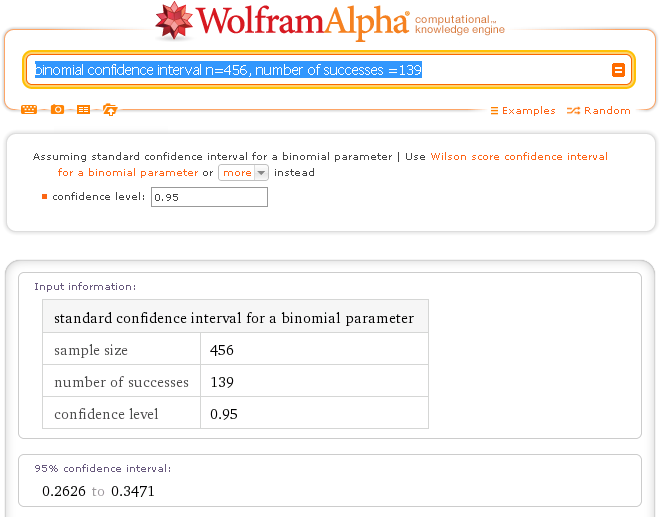
\includegraphics[width=12cm]{../fig/Tut08-06.png}
    \end{center}

\subsubsection*{Las proporciones como caso especial de variables cualitativas (factores).}

Tal vez te preguntes por qué en este caso no hemos incluido un fichero para trabajar con los datos de la muestra ``en bruto'' ({\em raw data}, en inglés). ¿Cómo sería el fichero del Ejemplo \ref{curso-cap08:ejem:IntervaloConfianzaProporcionAraos} del libro (pág. \pageref{curso-cap08:ejem:IntervaloConfianzaProporcionAraos}), el de los araos embridados? Tendría que ser una lista con $456$ valores como estos:
\begin{verbatim}
  embridado
  noEmbridado
  noEmbridado
  embridado
  noEmbridado
  embridado
  ...
\end{verbatim}
Las proporciones son variables de tipo Bernouilli y, por tanto, son simplemente respuestas de tipo sí/no. Por eso no hemos querido, artificiosamente, hacerte trabajar con ficheros que contengan $456$ filas de síes y noes. Es más fácil darte el resumen, como hemos hecho en ese ejemplo,  y decir {\em ``hay  139 araos embridados y 317 no embridados''.}

¡Pero cuidado! Eso no significa que no te vayas a encontrar con ficheros que contengan información sobre variables de tipo Bernouilli. Al contrario: es extremadamente frecuente. Porque, como hemos dicho ya varias veces a lo largo del curso, lo habitual es que se midan a la vez varias características en una misma observación. En la Figura \ref{curso-cap01:fig:DatosAlumnosCalc} del libro (pág. \pageref{curso-cap01:fig:DatosAlumnosCalc}), que reproducimos aquí, puedes ver algunas líneas del fichero {\tt  cap01-DatosAlumnos.csv},

\begin{center}
  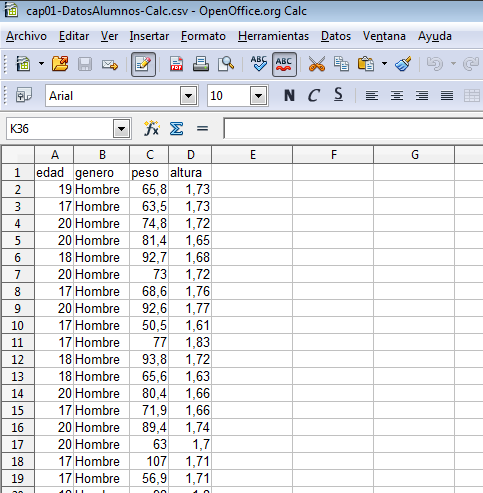
\includegraphics[height=10cm]{../fig/Cap01-DatosAlumnos.png}
\end{center}

La variable {\tt genero} de este fichero es una variable de Bernouilli, con sólo dos posibles variables y su papel en este conjunto de datos es una muestra típica de las situaciones en las que intervienen esas variables, que sirven para {\em clasificar} los datos en subgrupos. Por supuesto, todas las variables cualitativas (factores) sirven para esto, pero las variables tipo Bernouilli son especialmente sencillas, porque definen clasificaciones con sólo dos posibles clases.

En R, la forma natural de manejar un conjunto de datos como el de esta figura es mediante los {\tt data.frames} que hemos visto en el Tutorial04. Un {\tt data.frame} puede incluir una o varias variables de tipo Bernouilli en sus columnas. Y, en ese caso, si deseas hacer un intervalo de confianza para una de esas variables, sí que tendrás que trabajar a partir de los datos en bruto y hacer una tabla de frecuencias para obtener las proporciones muestrales. En la sección \ref{tut08:sec:FactoresR} de este tutorial vamos a avanzar en nuestra comprensión del trabajo con factores dentro de R.

\subsection{Contrastes de hipótesis para la proporción.}
\label{tut08:subsec:ContrastesHipotesisProporcion}

Para los contrastes de hipótesis podemos repetir el esquema básico que hemos visto para los intervalos.

\subsubsection*{Usando R.}

Empezamos con un fichero plantilla de R para este tipo de contrastes:
    \begin{center}
       \fichero{./code/Tut08-Contraste-Proporcion-UsandoZ.R}{Tut08-Contraste-Proporcion-UsandoZ.R}
    \end{center}


\begin{ejercicio}
\label{tut08:ejercicio02}
\begin{enumerate}
    \item[]
    \item Usa ese fichero para comprobar las cuentas del contraste de hipótesis que aparece en el Ejemplo \ref{curso-cap08:ejem:ContrasteHipotesisProporcionAraos} (pág. \pageref{curso-cap08:ejem:ContrasteHipotesisProporcionAraos}).
    \item Según el {\em Barómetro} del CIS de enero del 2013, en una muestra de 2452 personas residentes en España, 568 de ellas se declararon {\em no creyentes}. Usa estos datos para contrastar, al 95\%, la hipótesis de que la proporción de {\em no creyentes} es inferior al 25\%.
\end{enumerate}
Soluciones en la página \pageref{tut08:ejercicio02:sol}.
\qed
\end{ejercicio}

Como ya hemos adelantado, la función {\tt prop.test} está pensada para este tipo de contrastes. Como sucedía con {\tt t.test}, {\tt var.test} y otras funciones similares, el argumento {\tt alternative} nos permite seleccionar un contraste bilateral o unilateral y, en este segundo caso, si usamos la cola derecha o izquierda. Por ejemplo, el contraste del Ejemplo \ref{curso-cap08:ejem:ContrasteHipotesisProporcionAraos} (pág. \pageref{curso-cap08:ejem:ContrasteHipotesisProporcionAraos}) se obtiene así con {\tt prop.test}:

\begin{knitrout}
\definecolor{shadecolor}{rgb}{0.969, 0.969, 0.969}\color{fgcolor}\begin{kframe}
\begin{alltt}
\hlstd{(contraste} \hlkwb{=} \hlkwd{prop.test}\hlstd{(}\hlkwc{x}\hlstd{=}\hlnum{39}\hlstd{,} \hlkwc{n}\hlstd{=}\hlnum{105}\hlstd{,} \hlkwc{alternative} \hlstd{=} \hlstr{"greater"}\hlstd{,}
                      \hlkwc{p}\hlstd{=}\hlnum{0.35}\hlstd{,} \hlkwc{conf.level} \hlstd{=} \hlnum{0.95}\hlstd{,} \hlkwc{correct} \hlstd{=} \hlnum{FALSE}\hlstd{))}
\end{alltt}
\begin{verbatim}
## 
## 	1-sample proportions test without continuity correction
## 
## data:  39 out of 105, null probability 0.35
## X-squared = 0.212, df = 1, p-value = 0.32
## alternative hypothesis: true p is greater than 0.35
## 95 percent confidence interval:
##  0.29801 1.00000
## sample estimates:
##       p 
## 0.37143
\end{verbatim}
\end{kframe}
\end{knitrout}
Recuerda que {\tt greater} se usa cuando $H_a=\{p > p_0\}$, que {\tt less} se usa con $H_a=\{p < p_0\}$ y que {\tt two.sided} se usa con $H_a=\{p \neq p_0\}$.

Por razones técnicas, que quedarán más claras en el Capítulo \ref{curso-cap:TablasContingenciaTestChi2} del libro, el estadístico que obtenemos en {\tt prop.test}, y que aparece como {tt X-squared}, es en realidad el cuadrado del que obtendrás si usas el fichero plantilla que hemos visto antes. Además, hemos usado la opción {\tt correct=FALSE} por las mismas razones que discutimos en el caso de los intervalos de confianza.


\subsubsection*{Usando GeoGebra.}

En la {\em Calculadora  de Probabilidades} de GeoGebra tenemos la posibilidad de realizar uno de estos contrastes, dentro de la pestaña {\em Estadísticas}, como se muestra en la figura:
\begin{center}
    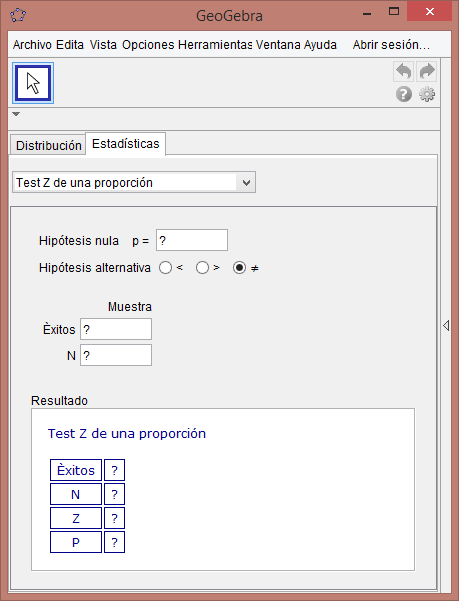
\includegraphics[width=7cm]{../fig/Tut08-01.png}
\end{center}

\begin{ejercicio}
\label{tut08:ejercicio03}
Usa GeoGebra para repetir el Ejercicio \ref{tut08:ejercicio02}. Solución en la página \pageref{tut08:ejercicio03:sol}.
\qed
\end{ejercicio}


%\subsection{Con otros programas}
\subsubsection*{Usando Wolfram Alpha.}

En Wolfram Alpha podemos usar el comando

{\tt proportion hypothesis test}

para llegar a un interfaz en el que introducir los valores necesarios para el contraste, que se muestra en esta figura:
\begin{center}
    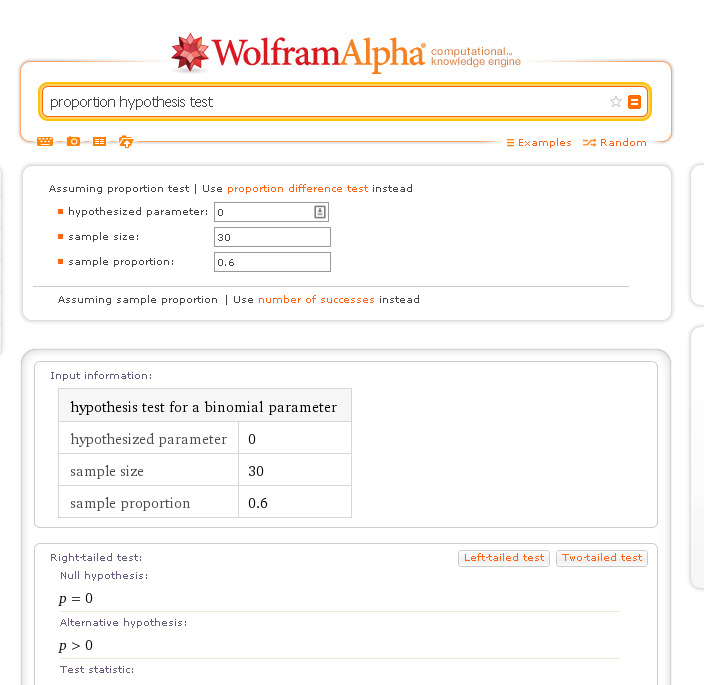
\includegraphics[width=13cm]{../fig/Tut08-07.png}
\end{center}


\section{Intervalos de confianza exactos para la proporción. Método de Clopper-Pearson.}
\label{tut08:sec:MetodoExactoBinomial}
\noindent {\bf Atención:} Esta sección es opcional en una primera lectura.\\

La Sección \ref{curso-cap08:subsec:MetodoExactoBinomial} del libro (pág. \pageref{curso-cap08:subsec:MetodoExactoBinomial}) describe él método exacto de Clopper-Pearson para hacer inferencia sobre proporciones en casos que no cubre la aproximación por la distribución normal.  En esta breve sección sólo queremos comentar que R dispone de la función {\tt binom.test}, que permite obtener este tipo de resultados de una forma muy cómoda.

La forma de usar {\tt binom.test} nos debe resultar muy familiar a estas alturas, porque se comporta de manera similar a {\t t.test} y funciones semejantes. A modo de ilustración, para obtener los resultados del Ejemplo \ref{curso-cap08:ejem:ContrasteHipotesisProporcionClopperPearson} del libro (pág. \pageref{curso-cap08:ejem:ContrasteHipotesisProporcionClopperPearson}) usaríamos {\tt binom.test} de esta manera:

\begin{knitrout}
\definecolor{shadecolor}{rgb}{0.969, 0.969, 0.969}\color{fgcolor}\begin{kframe}
\begin{alltt}
\hlkwd{binom.test}\hlstd{(}\hlkwc{x} \hlstd{=} \hlnum{2}\hlstd{,} \hlkwc{n} \hlstd{=} \hlnum{15}\hlstd{,} \hlkwc{p} \hlstd{=} \hlnum{0.1}\hlstd{,} \hlkwc{alternative} \hlstd{=} \hlstr{"greater"}\hlstd{,} \hlkwc{conf.level} \hlstd{=} \hlnum{0.95}\hlstd{)}
\end{alltt}
\begin{verbatim}
## 
## 	Exact binomial test
## 
## data:  2 and 15
## number of successes = 2, number of trials = 15, p-value = 0.45
## alternative hypothesis: true probability of success is greater than 0.1
## 95 percent confidence interval:
##  0.024226 1.000000
## sample estimates:
## probability of success 
##                0.13333
\end{verbatim}
\end{kframe}
\end{knitrout}

Como ves, el p-valor coincide con el que aparece en el Ejemplo \ref{curso-cap08:ejem:ContrasteHipotesisProporcionClopperPearson}. Además, como subproducto del cálculo obtenemos un intervalo de confianza para la proporción. Pero ten en cuenta que como la hipótesis alternativa es unilateral, ese intervalo es también unilateral. Si se desea un intervalo de confianza bilateral, debemos usar la opción {\tt two.sided} en {\tt binom.test}. Así, el intervalo de confianza del Ejemplo \ref{curso-cap08:ejem:ContrasteHipotesisProporcionClopperPearson2} del libro (pág. \pageref{curso-cap08:ejem:ContrasteHipotesisProporcionClopperPearson2}) se obtiene con:

\begin{knitrout}
\definecolor{shadecolor}{rgb}{0.969, 0.969, 0.969}\color{fgcolor}\begin{kframe}
\begin{alltt}
\hlkwd{binom.test}\hlstd{(}\hlkwc{x} \hlstd{=} \hlnum{2}\hlstd{,} \hlkwc{n} \hlstd{=} \hlnum{15}\hlstd{,} \hlkwc{p} \hlstd{=} \hlnum{0.1}\hlstd{,} \hlkwc{alternative} \hlstd{=} \hlstr{"two.sided"}\hlstd{,} \hlkwc{conf.level} \hlstd{=} \hlnum{0.95}\hlstd{)}
\end{alltt}
\begin{verbatim}
## 
## 	Exact binomial test
## 
## data:  2 and 15
## number of successes = 2, number of trials = 15, p-value = 0.66
## alternative hypothesis: true probability of success is not equal to 0.1
## 95 percent confidence interval:
##  0.016576 0.404603
## sample estimates:
## probability of success 
##                0.13333
\end{verbatim}
\end{kframe}
\end{knitrout}

Naturalmente, también es posible construir estos intervalos directamente, usando {\tt pbinom} o una herramienta análoga, y siguiendo los pasos que se describen el el libro. Eso abre la puerta al cálculo de estos contrastes e intervalos usando otros programas como GeoGebra, Wolfram Alpha o, en general, cualquier programa que permita calcular probabilidades binomiales. No nos vamos a extender más aquí sobre el tema.


%En los apartados anteriores hemos usado la aproximación de la binomial por la normal para realizar
%inferencia, tanto en el caso de los intervalos de confianza, como en el de los contrastes de
%hipótesis. Pero debemos tener presente que hay casos en los que esa aproximación no es posible,
%porque no se cumplen las condiciones necesarias. En particular, eso sucede cuando $p$ es muy
%pequeño, caso que veremos en la Sección \ref{curso-cap08:sec:DistribucionPoisson}, o cuando las
%muestras son pequeñas.  Aquí vamos a fijarnos especialmente en el caso de muestras de tamaño
%pequeño.  Al usar la normal para muestras de tamaño grande, lo que hemos estado haciendo es una
%{\em aproximación}. Por lo tanto, es posible preguntarse si, para trabajar con muestras pequeñas,
%podríamos utilizar un método {\em exacto}. ¿Qué quiere decir esto? Que, en lugar de la normal,
%usamos la distribución binomial directamente.  Este método, para que nuestro trabajo tenga un
%mínimo de precisión, presupone que somos capaces de calcular valores de probabilidad binomial de
%forma efectiva. Por eso, este tipo de métodos son especialmente interesantes cuando se emplea un
%ordenador.
%
%Vamos discutir aquí, como de costumbre informalmente, el punto de partida de este método. Y
%dejaremos la parte práctica para el Tutorial08, en el que veremos como usar R para estos cálculos.
%Una referencia habitual para estos métodos (y para la crítica que puede hacerse de ellos) es el
%artículo de Agresti y Coull \cite{agresti1998approximate}.
%
%Empecemos. En cada ejemplo concreto, tendremos una población en la que, como hemos discutido en los
%apartados anteriores, hay definida una variable de Bernouilli (éxito/fracaso). Para usar una
%notación más clara, en lo que sigue,  supondremos que $p_0$ es el {\em valor real} de la proporción
%en la población. Por lo tanto la población es una variable de tipo {\em Bernouilli$(p_0)$}. Nuestro
%objetivo, como antes, es estimar el parámetro $p_0$ de la población. Como de costumbre, usaremos
%una muestra aleatoria, formada por $n$ observaciones independientes de esa población. Vamos a
%llamar $k$ al número de éxitos (en el sentido de la binomial) que contiene la muestra. Es decir,
%que la proporción muestral, en el lenguaje que venimos usando, vale, en esa muestra:
%\[\hat p=\dfrac{k}{n}.\]
%Y vimos, al principio de este capítulo, que la proporción muestral sigue una distribución
%    \[\hat p \sim {\dfrac{1}{n}}B(n,p_0).\]
%Esto es lo mismo que decir que la variable $k=n\cdot \hat p$, que mide el número de éxitos en la
%muestra, sigue una distribución binomial $B(n,p_0)$. En esta situación vamos a considerar $n$ como
%un dato del problema, y $k$ como una variable que puede tomar cualquier valor de $0$ a $n$, cuando
%recorremos el espacio de todas las posibles muestras de tamaño $n$.
%
%Teniendo todo esto en cuenta, nuestro objetivo es el siguiente: tomamos un nivel de confianza $nc$.
%Para fijar ideas, en el resto de la discusión vamos a usar  $nc=0.95$. Se trata, entonces, de usar
%$n$ y $k$ para obtener un intervalo de confianza $(p_1, p_2)$ {\em que contenga a $p_0$ el $95\%$
%de las veces.}
%
%¿Qué queremos decir con este ``95\% de las veces''? Recuerda que desconocemos el valor de $p_0$.
%Así que lo nos gustaría es garantizar que, sea cual sea $p_0$, en el $95\%$ de los casos posibles,
%donde cada caso corresponde a una posible muestra de tamaño $n$, nuestro procedimiento producirá
%como resultado un intervalo de confianza, que contendrá el valor real de $p_0$.  Así que la
%probabilidad del $95\%$, de la que hemos hablado, se refiere a probabilidad sobre todos las
%posibles muestras de tamaño $n$, suponiendo que la probabilidad real es $p_0$. Como en otros casos,
%el $95\%$ se refiere al espacio muestral asociado al problema que estamos considerando.
%
%Así que, concretando más, lo que vamos a hacer es definir un procedimiento, que a partir de los
%valores de la muestra, produzca los números $p_1$ y $p_2$. Esquemáticamente,
%\[  (n,k) \dashrightarrow (p_1,p_2)\]
%y queremos garantizar que:
%\begin{equation}\label{tut08:ecu:CondicionProbabilidadClopperPearson}
%P(p_1 < p_0 < p_2)> 0.95,
%\end{equation}
%en el sentido que hemos explicado. Fíjate en que hemos escrito \[>0.95,\] y no \[=0.95\] como en
%otros intervalos que hemos discutido antes en el curso. Al hacer esto estamos garantizando el nivel
%de confianza que queremos, aunque el intervalo pueda resultar un poco más ancho de lo necesario.
%
%Para conseguir que ocurra esto, tenemos que pensar un poco más sobre la condición
%\ref{tut08:ecu:CondicionProbabilidadClopperPearson}. La condición se puede reescribir así, en
%términos de $\alpha$ (la desigualdad se invierte):
%\[\left(1-P(p_1 < p_0 < p_2)\right)\,  < \, (1-0.95)\, =\,\alpha=0.05.\]
%Y hay que tener en cuenta que $p_1 < p_0 < p_2$ significa lo mismo que la intersección:
%\[(p_1 < p_0) \cap (p_0< p_2).\]
%El suceso contrario de esa intersección es:
%\[(p_0\leq p_1) \cup (p_2 \leq p_0),\]
%Ahora, tengamos en cuenta que, puesto que vamos que hacer que se cumpla $p_1<p_2$, las condiciones
%$(p_0\leq p_1) $ y $(p_2 \leq p_0)$ son disjuntas (incompatibles). Así que la propiedad de la
%probabilidad de la unión (pág. \pageref{cap03:def:PropiedadesFundamentalesFuncionProbabilidad}),
%aplicada a este caso permite escribir:
%\[\alpha > 1-P(p_1 < p_0 < p_2) =
%P\left((p_0 \leq p_1) \cup (p_2\leq p_0)\right) = P\left(p_0 \leq p_1\right)+ P\left(p_0\geq p_2\right),\]
%donde, en el último término, hemos escrito al revés la segunda desigualdad. La suma de estos dos
%términos tiene que ser, a lo sumo, $\alpha$, así que (como hicimos en el caso de $\chi^2$) vamos a
%pedir que cada uno de ellos sume, como mucho, $\alpha/2$. Es decir que, para construir el intervalo
%de confianza, vamos a buscar valores $p_1$ y $p_2$ tales que:
%\[
%\begin{cases}
%P\left(p_0 \leq p_1\right)<0.025\\
%P\left(p_0 \geq p_2\right)<0.025
%\end{cases}
%\]
%o, de otro modo:
%\begin{equation}\label{tut08:ecu:CondicionProbabilidadClopperPearson02}
%\begin{cases}
%P\left(p_0 \geq p_1\right)\geq 0.025\\
%P\left(p_0 \leq p_2\right)\geq 0.025
%\end{cases}
%\end{equation}
%Ese es el objetivo a conseguir. Volvamos ahora a la muestra, caracterizada por $n$ y $k$, y vamos a
%ver cómo se usan $n$ y $k$ para calcular los valores $p_1$ y $p_2$. Consideramos a $p$ como una
%variable en el intervalo $(0,1)$ y sea $X$ una variable binomial de tipo $B(n,p)$.
%
%Empezaremos calculando $p_2$. Usemos $p$ como variable, para localizar el subconjunto $A$ de
%valores en el intervalo $0\leq p\leq 1$ para los que se cumple esta condición:
%\[
%P\left(  X\leq  k \right)>0.025
%\]
%(recuerda que $k$ es el número de éxitos en la muestra).  ¿Qué tiene que ver esto con la segunda
%condición en la Ecuación \ref{tut08:ecu:CondicionProbabilidadClopperPearson02}? La desigualdad
%$X\leq k$ está escrito en términos de ``número de éxitos'', mientras que en
%\ref{tut08:ecu:CondicionProbabilidadClopperPearson02} hablábamos de proporciones. Así que basta con
%dividir los dos términos de $X\leq k$ por $n$ para ver la relación entre ambas condiciones.
%
%Para ver como funciona esto en detalle, pensemos en lo que sucede cuando $p$ aumenta desde $0$
%hasta $1$. Observa que si $p=0$ (es imposible obtener un éxito), es decir,  $X\sim B(n,0)$,
%entonces $X$ siempre vale $0$, y sea cual sea $k$
%\[
%P\left(  X\leq  k \right)=1.
%\]
%Por el contrario, si $p=1$ (todo son éxitos), entonces $X=n$ y
%\[
%P\left(  X\leq k \right)=0
%\]
%salvo que sea $k=n$. Así que, a medida que aumentamos $p$ desde $0$ hasta $1$, la probabilidad
%$P\left(X\leq k \right)$ disminuye de 1 a 0. Entonces habrá  un valor $p_2$ para el que, si
%$p>p_2$, se cumplirá
%\[
%P\left(  X\leq  k \right)>0.025
%\]
%En el caso $k=0$, tomamos $p_2=1$. En cualquier caso, el resumen es que $A=\{p | P\left(  X\leq  k
%\right)>0.025 \}=[0,p_2]$.
%
%De la misma forma, vamos a localizar el subconjunto $B$ de valores del intervalo $0\leq p\leq 1$
%para los que se cumple esta condición:
%\[
%P\left(  X\geq  k \right)>0.025
%\]
%Ahora, cuando $p$ aumenta desde $0$ hasta $1$, las cosas van al revés. Si $p=0$ (es imposible
%obtener un éxito), entonces $X$ siempre vale $0$, y
%\[
%P\left(  X\geq  k \right)=0.
%\]
%salvo para, precisamente, $k=0$. Por contra, cuando $p=1$,  todo son éxitos, $X$ siempre vale $n$,
%y sea cual sea $k$
%\[
%P\left(  X\geq  k \right)=1.
%\]
%En el caso $k=0$, tomaremos $p_1=0$. Se deduce que el subconjunto $B$ que buscábamos es de la
%forma: $B=\{p | P\left(  X\geq  k \right)>0.025 \}=[p_1,1]$.
%
%Con eso, hemos localizado $p_1$ y $p_2$. El intervalo de confianza es, entonces, el conjunto
%\[A\cap B= [p_1,1]\cap [0,p_2] = [p_1,p_2].\]
%Insistimos en que, en el Tutorial08, veremos cómo hacer eso en la práctica. Ahora, vamos a
%comprobar que este intervalo tiene las propiedades deseadas.
%
%Supongamos entonces que $p_0$ es la probabilidad de la población y que hemos obtenido una muestra
%de tamaño $n$ con $k$ éxitos. Usamos esa muestra para construir el intervalo de confianza
%$[p_1,p_2]$ por el procedimiento que hemos descrito más arriba. ¿Qué tendría que suceder para que
%$p_0$ no perteneciera a $[p_1,p_2])$? Sea $X$ la binomial $B(n,p_0)$. Tendría entonces que suceder
%una de estas dos cosas:
%\[P\left(  X\geq  k \right)<0.025\]
%o
%\[P\left(  X\leq  k \right)<0.025\]
%Estas dos desigualdades implican que, en conjunto, las posibles muestras con valores $k$ para los
%que esto sucede, no representan, en probabilidad, más que $0.025+0.025=0.05$. Es decir, que para al
%menos el $95\%$ de las posibles muestras, el intervalo que hemos construido contiene a $p_0$, como
%pretendíamos.


\section{La distribución de Poisson}
\label{tut08:sec:DistribucionPoisson}

En la sección \ref{curso-cap08:sec:DistribucionPoisson} del libro (pág. \pageref{curso-cap08:sec:DistribucionPoisson}) se presenta la distribución de Poisson, y se explica el papel que juega esta distribución como una alternativa para aquellos casos en que tendríamos que trabajar con una distribución binomial con $n$ grande pero a la vez $p$ pequeño. Aquí vamos a ver algunas herramientas computacionales útiles para trabajar con esa distribución.

\subsection{La distribución de Poisson en R.}

Para trabajar con la distribución de Poisson disponemos en R de cuatro funciones análogas a las que vimos en el caso de la distribución binomial:
    \begin{center}
    \begin{minipage}{10cm}
    \begin{verbatim}
    dpois     ppois     qpois     rpois
    \end{verbatim}
    \end{minipage}
    \end{center}
Suponemos que, a estas alturas, es fácil intuir la finalidad y funcionamiento de todas ellas. Vamos a comentarlas por tanto brevemente, deteniéndonos sólo en los aspectos que pueden plantear alguna dificultad:
\begin{itemize}

  \item {\tt dpois} es la función de densidad, y por lo tanto, si $X$ es una variable de tipo
      $\operatorname{Pois}(\lambda)$, pongamos por ejemplo con $\lambda=5$, entonces para
      calcular:
      \[P(X=7),\]
      ejecutaríamos este comando:
\begin{knitrout}
\definecolor{shadecolor}{rgb}{0.969, 0.969, 0.969}\color{fgcolor}\begin{kframe}
\begin{alltt}
\hlkwd{dpois}\hlstd{(}\hlnum{7}\hlstd{,} \hlkwc{lambda}\hlstd{=}\hlnum{5}\hlstd{)}
\end{alltt}
\begin{verbatim}
## [1] 0.10444
\end{verbatim}
\end{kframe}
\end{knitrout}

  \item {\tt ppois} nos permite calcular la probabilidad de la cola izquierda de una distribución de Poisson. Y como en el caso de la binomial, al tratarse de una {\bf distribución discreta}, tenemos que ser cuidadosos. La cola izquierda aquí se define usando la desigualdad $\leq$. Es decir, que si, como antes, $\lambda=5$, entonces para calcular
      \[P(X\leq 4),\]
      debemos ejecutar:
\begin{knitrout}
\definecolor{shadecolor}{rgb}{0.969, 0.969, 0.969}\color{fgcolor}\begin{kframe}
\begin{alltt}
\hlkwd{ppois}\hlstd{(}\hlnum{4}\hlstd{,} \hlkwc{lambda}\hlstd{=}\hlnum{5}\hlstd{)}
\end{alltt}
\begin{verbatim}
## [1] 0.44049
\end{verbatim}
\end{kframe}
\end{knitrout}
      Mientras que, si lo que queremos es calcular la probabilidad con una desigualdad estricta,
      debemos convertirla primero en no estricta, como en este ejemplo:
      \[P(X<4) = P(X\leq 3),\]
      y ahora calcular
\begin{knitrout}
\definecolor{shadecolor}{rgb}{0.969, 0.969, 0.969}\color{fgcolor}\begin{kframe}
\begin{alltt}
\hlkwd{ppois}\hlstd{(}\hlnum{3}\hlstd{,} \hlkwc{lambda}\hlstd{=}\hlnum{5}\hlstd{)}
\end{alltt}
\begin{verbatim}
## [1] 0.26503
\end{verbatim}
\end{kframe}
\end{knitrout}
      Para calcular la probabilidad de una cola derecha
      hay que usar, como de costumbre {\tt 1-ppois} o la opción {\tt lower.tail=FALSE}, con las mismas precauciones al tratarse de
      una distribución discreta.

  \item {\tt qpois} sirve para resolver problemas inversos de probabilidad, usando la cola izquierda y una desigualdad no estricta $\leq$. Además, debe tenerse en cuenta que, puesto que se trata de una variable discreta, los problemas inversos se definen, en general, como desigualdades sobre la probabilidad. Es decir, que por ejemplo, si $X$ es de tipo
      $\operatorname{Pois}(15)$ (es decir, $\lambda=15$), y  buscamos el valor $a$ que tiene la
      propiedad de que:
      \[P(X\leq a)=0.35\]
      Es muy posible que ninguno de los posibles valores de $X$ (que son los números naturales
      $0, 1, 2,\ldots$) tenga esa propiedad. Si, en cambio, preguntamos por el primer valor (el valor más pequeño) para  el que se cumple:
      \[P(X\leq a)\geq 0.35\]
      entonces la pregunta está bien definida, y la respuesta se obtiene con
\begin{knitrout}
\definecolor{shadecolor}{rgb}{0.969, 0.969, 0.969}\color{fgcolor}\begin{kframe}
\begin{alltt}
\hlkwd{qpois}\hlstd{(}\hlnum{0.35}\hlstd{,} \hlkwc{lambda}\hlstd{=}\hlnum{15}\hlstd{)}
\end{alltt}
\begin{verbatim}
## [1] 13
\end{verbatim}
\end{kframe}
\end{knitrout}
      Y puedes comprobarlo calculando la probabilidad acumulada para ese valor (el $13$) y para los valores adyacentes $12$ y $14$.
\begin{knitrout}
\definecolor{shadecolor}{rgb}{0.969, 0.969, 0.969}\color{fgcolor}\begin{kframe}
\begin{alltt}
\hlkwd{ppois}\hlstd{(}\hlnum{12}\hlopt{:}\hlnum{14}\hlstd{,} \hlkwc{lambda}\hlstd{=}\hlnum{15}\hlstd{)}
\end{alltt}
\begin{verbatim}
## [1] 0.26761 0.36322 0.46565
\end{verbatim}
\end{kframe}
\end{knitrout}

  \item {\tt rpois} sirve para obtener valores aleatorios de una distribución de Poisson y se usa, sobre todo, para realizar simulaciones.

\end{itemize}

\subsubsection*{Usando GeoGebra.}

En GeoGebra puedes usar la calculadora de Probabilidades en la forma habitual para resolver problemas de probabilidad directos e inversos que involucren a la distribución de Poisson. La siguiente figura muestra la interfaz de la calculadora mientras resolvemos uno de esos problemas.

\begin{center}
    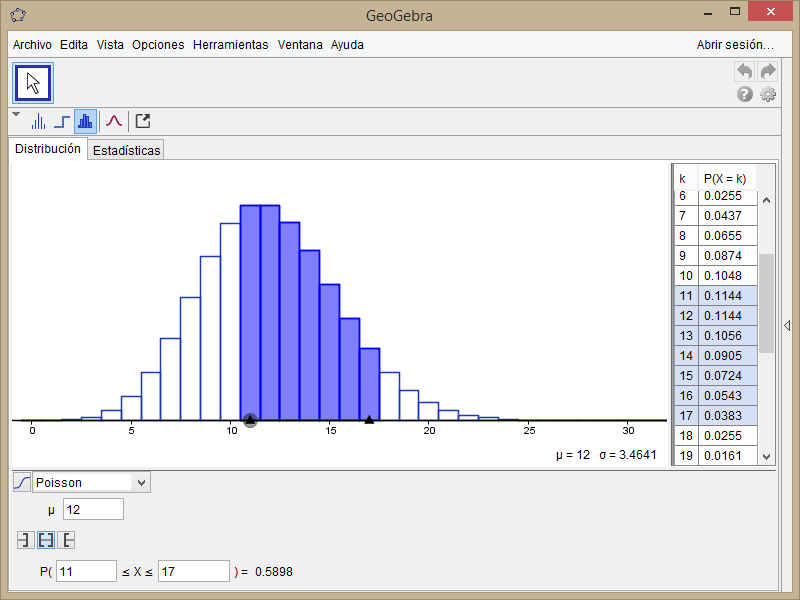
\includegraphics[width=15cm]{../fig/Tut08-02.png}
\end{center}

Aparte de esto, si utilizas la {\em Línea de entrada} o el panel de {\em Cálculo Simbólico} puedes usar, en cualquiera de ellos, los comandos:
\begin{verbatim}
  Poisson[ <Media>, <Valor>, <Acumulada o no (true/false)> ]
  PoissonInversa[ <Media>, <Probabilidad> ]
  PoissonAleatoria[ <Media> ]
\end{verbatim}
La {\tt media} es el valor de $\lambda$, claro. El comando {\tt Poisson} condensa las funcionalidades que en R se obtienen con {\tt dpois} y {\tt ppois}. Debes usar la opción {\em Acumulada} para elegir:
 \begin{itemize}
   \item entre la función de distribución (como {\tt ppois} en R) cuando {\em Acumulada} es {\tt true}
   \item y la función de densidad (como {\tt dpois} en R) cuando es {\tt false}.
 \end{itemize}
{\tt PoissonInversa} se comporta de forma similar a {\tt qpois} (también con la cola izquierda), mientras que {\tt PoissonAleatoria} devuelve un único valor aleatorio de la distribución de Poisson.

\subsubsection*{Usando Wolfram Alpha.}

Para realizar cálculos de probabilidad directa con la distribución de Poisson, podemos usar comandos como este:
\begin{verbatim}
  P[4<X] for X~Poisson(3)
\end{verbatim}
cuyo equivalente en R es:
\begin{knitrout}
\definecolor{shadecolor}{rgb}{0.969, 0.969, 0.969}\color{fgcolor}\begin{kframe}
\begin{alltt}
\hlnum{1} \hlopt{-} \hlkwd{ppois}\hlstd{(}\hlnum{4}\hlstd{,} \hlkwc{lambda}\hlstd{=}\hlnum{3}\hlstd{)}
\end{alltt}
\begin{verbatim}
## [1] 0.18474
\end{verbatim}
\end{kframe}
\end{knitrout}
El resultado en Wolfram Alpha se muestra en la siguiente figura:
\begin{center}
    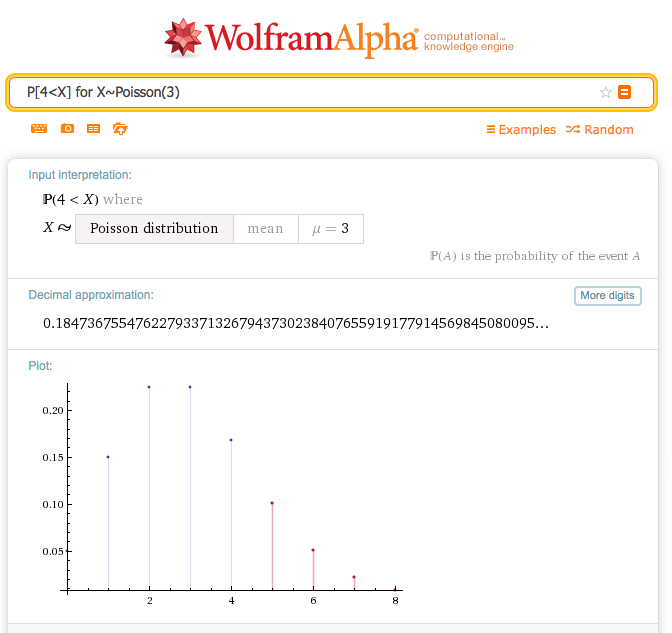
\includegraphics[width=12cm]{../fig/Tut08-03.png}
\end{center}

Mientras que
\begin{verbatim}
  InverseCDF[Poisson(4), 0.75]
\end{verbatim}
es el equivalente en Wolfram Alpha del comando de R
\begin{knitrout}
\definecolor{shadecolor}{rgb}{0.969, 0.969, 0.969}\color{fgcolor}\begin{kframe}
\begin{alltt}
\hlkwd{qpois}\hlstd{(}\hlnum{0.75}\hlstd{,} \hlkwc{lambda}\hlstd{=}\hlnum{4}\hlstd{)}
\end{alltt}
\begin{verbatim}
## [1] 5
\end{verbatim}
\end{kframe}
\end{knitrout}
Aquí {\tt CDF} es una abreviatura de {\em cumulative distribution function} o {\em función de distribución acumulada}, lo que nosotros llamamos simplemente {\em función de distribución}.

\begin{center}
    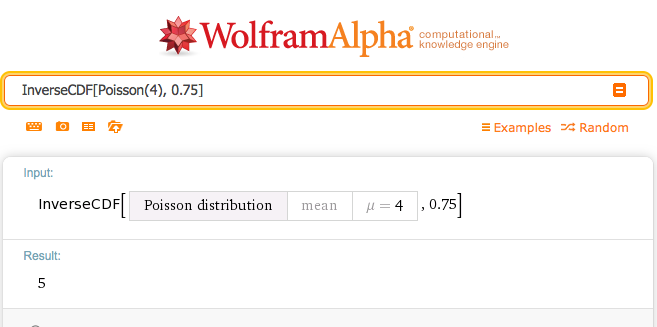
\includegraphics[width=12cm]{../fig/Tut08-04.png}
\end{center}

\begin{ejercicio}
\label{tut08:ejercicio04}
\begin{enumerate}
  \item[]
  \item Comprueba los cálculos de probabilidad del Ejemplo \ref{curso-cap08:ejem:Poisson01} del libro (pág. \pageref{curso-cap08:ejem:Poisson01}) usando R, GeoGebra y Wolfram Alpha.
  \item  Comprueba también los cálculos de probabilidad del Ejemplo \ref{curso-cap08:ejem:PoissonMuertesInfarto02} del libro (pág. \pageref{curso-cap08:ejem:PoissonMuertesInfarto02}). En este caso, te recomendamos que uses R.
\end{enumerate}
Soluciones en la página \pageref{tut08:ejercicio04:sol}.
\qed
\end{ejercicio}



\subsection{Procesos de Poisson.}
\noindent{\bf Opcional: esta sección puede omitirse en una primera lectura.}


En esta sección nos vamos a limitar a incluir el código en R que te va a permitir reconstruir cálculos como los de la Sección \ref{curso-cap08:subsec:ProcesosPoisson} del libro (pág. \pageref{curso-cap08:subsec:ProcesosPoisson}).

Puesto que vamos a simular algunos valores, empezamos fijando la semilla del generador de números aleatorios de R.

\begin{knitrout}
\definecolor{shadecolor}{rgb}{0.969, 0.969, 0.969}\color{fgcolor}\begin{kframe}
\begin{alltt}
\hlkwd{set.seed}\hlstd{(}\hlnum{2013}\hlstd{)}
\end{alltt}
\end{kframe}
\end{knitrout}

A continuación introducimos los datos del INE sobre muertes por infarto en España en el año $2011$, calculamos la tasa por habitante y la usamos para {\em estimar} el número de muertes en Madrid.

\begin{knitrout}
\definecolor{shadecolor}{rgb}{0.969, 0.969, 0.969}\color{fgcolor}\begin{kframe}
\begin{alltt}
\hlstd{poblacionPais} \hlkwb{=} \hlnum{47190493}
\hlstd{muertesInfarto} \hlkwb{=} \hlnum{18101}

\hlstd{(probAnualMuerteInfarto} \hlkwb{=} \hlstd{muertesInfarto}\hlopt{/}\hlstd{poblacionPais  )}
\end{alltt}
\begin{verbatim}
## [1] 0.00038357
\end{verbatim}
\begin{alltt}
\hlstd{poblacionMadrid} \hlkwb{=} \hlnum{6489680}
\hlstd{(muertosAnualesInfartoMadrid} \hlkwb{=} \hlstd{poblacionMadrid} \hlopt{*} \hlstd{probAnualMuerteInfarto)}
\end{alltt}
\begin{verbatim}
## [1] 2489.3
\end{verbatim}
\end{kframe}
\end{knitrout}

A continuación empecemos con la primera simulación que se describe en el libro. Primero calculamos la probabilidad de que un madrileño cualquiera muera de infarto un día cualquiera de $2011$:

\begin{knitrout}
\definecolor{shadecolor}{rgb}{0.969, 0.969, 0.969}\color{fgcolor}\begin{kframe}
\begin{alltt}
\hlstd{Dias} \hlkwb{=} \hlnum{365}
\hlstd{(probDiariaMuerteInfarto} \hlkwb{=} \hlstd{probAnualMuerteInfarto}\hlopt{/}\hlnum{365}\hlstd{)}
\end{alltt}
\begin{verbatim}
## [1] 0.0000010509
\end{verbatim}
\end{kframe}
\end{knitrout}
Naturalmente,  esta simulación es una simplificación poco realista.  Estamos suponiendo que esa probabilidad es la misma para un saludable atleta de $20$ años que para un oficinista sedentario de $50$ años con antecedentes familiares de enfermades coronarias...

Pero en aras del modelo ignoremos por el momento esa falta de realismo y sigamos adelante. Vamos a usar esa probabilidad  para simular el número de madrileños que mueren en cada uno de los 365 días del año. Lo haremos calcuando $365$ valores de la correspondiente binomial, una binomial para cada día del año. Cada una de esas binomiales es $B(n, p)$ siendo $n$ el número de habitantes de Madrid y $p$ la probabilidad diaria de muerte por infarto para cada uno de ellos. Así que la simulación es:

\begin{knitrout}
\definecolor{shadecolor}{rgb}{0.969, 0.969, 0.969}\color{fgcolor}\begin{kframe}
\begin{alltt}
\hlstd{recuentoAnual} \hlkwb{=} \hlkwd{numeric}\hlstd{(Dias)}
\hlstd{p} \hlkwb{=} \hlstd{probDiariaMuerteInfarto}
\hlkwa{for}\hlstd{(i} \hlkwa{in} \hlnum{1}\hlopt{:}\hlnum{365}\hlstd{)\{}
  \hlstd{(casosDia} \hlkwb{=} \hlkwd{rbinom}\hlstd{(}\hlnum{1}\hlstd{,} \hlkwc{size}\hlstd{=poblacionMadrid,} \hlkwc{prob}\hlstd{=p))}
  \hlstd{recuentoAnual[i]} \hlkwb{=} \hlstd{casosDia}
\hlstd{\}}
\end{alltt}
\end{kframe}
\end{knitrout}

Y en esta simulación (distinta de la que aparece en el libro) obtenemos  esta tabla de frecuencias:
\begin{knitrout}
\definecolor{shadecolor}{rgb}{0.969, 0.969, 0.969}\color{fgcolor}\begin{kframe}
\begin{alltt}
\hlkwd{table}\hlstd{(recuentoAnual)}
\end{alltt}
\begin{verbatim}
## recuentoAnual
##  1  2  3  4  5  6  7  8  9 10 11 12 13 14 
##  5  9 24 34 50 49 60 46 30 29 16  8  4  1
\end{verbatim}
\end{kframe}
\end{knitrout}
La primera fila indica el número de fallecimientos por día y la segunda el número de días del año en los que se produjo esa cifra. Como ves el número más frecuente de muertes por infarto y por día es $7$. En esta simulación ese número de muertes ha ocurrido en $60$ de los $365$ días posibles. Pero también hay $5$ días con una única muerte y un día con $14$ muertes. El número total de muertes en todo el año y para esta simulación asciende a:
\begin{knitrout}
\definecolor{shadecolor}{rgb}{0.969, 0.969, 0.969}\color{fgcolor}\begin{kframe}
\begin{alltt}
\hlkwd{sum}\hlstd{(recuentoAnual)}
\end{alltt}
\begin{verbatim}
## [1] 2461
\end{verbatim}
\end{kframe}
\end{knitrout}
¡No nos cansamos de repetir que es una simulación y que no pretende reproducir el número real observado ese año!

Para seguir adelante, en lugar de días usamos horas. El número de horas en un año es
\begin{knitrout}
\definecolor{shadecolor}{rgb}{0.969, 0.969, 0.969}\color{fgcolor}\begin{kframe}
\begin{alltt}
\hlstd{(Horas} \hlkwb{=} \hlstd{Dias} \hlopt{*} \hlnum{24}\hlstd{)}
\end{alltt}
\begin{verbatim}
## [1] 8760
\end{verbatim}
\end{kframe}
\end{knitrout}
y la probabilidad de muerte individual por hora para un madrileño se calcula así:
\begin{knitrout}
\definecolor{shadecolor}{rgb}{0.969, 0.969, 0.969}\color{fgcolor}\begin{kframe}
\begin{alltt}
\hlstd{(probHoraMuerteInfarto} \hlkwb{=} \hlstd{probDiariaMuerteInfarto} \hlopt{/} \hlnum{24}\hlstd{)}
\end{alltt}
\begin{verbatim}
## [1] 4.3787e-08
\end{verbatim}
\end{kframe}
\end{knitrout}
Y ahora hacemos otra nueva simulación, esta vez con $8760$ binomiales (una por hora), cada una de ellas con $n$ igual al número de habitantes de Madrid pero ahora con $p$ igual a la probabilidad {\em horaria} de muerte por infarto para cada madrileño.
\begin{knitrout}
\definecolor{shadecolor}{rgb}{0.969, 0.969, 0.969}\color{fgcolor}\begin{kframe}
\begin{alltt}
\hlstd{recuentoAnual}\hlkwb{=}\hlkwd{numeric}\hlstd{(Horas)}
\hlstd{(p}\hlkwb{=}\hlstd{probHoraMuerteInfarto)}
\end{alltt}
\begin{verbatim}
## [1] 4.3787e-08
\end{verbatim}
\begin{alltt}
\hlkwa{for}\hlstd{(i} \hlkwa{in} \hlnum{1}\hlopt{:}\hlstd{Horas)\{}
  \hlstd{(casosHora}\hlkwb{=}\hlkwd{rbinom}\hlstd{(}\hlnum{1}\hlstd{,}\hlkwc{size}\hlstd{=poblacionMadrid,}\hlkwc{prob}\hlstd{=p))}
  \hlstd{recuentoAnual[i]}\hlkwb{=}\hlstd{casosHora}
\hlstd{\}}
\end{alltt}
\end{kframe}
\end{knitrout}
La correspondiente tabla y el total de muertes en esta simulación son:
\begin{knitrout}
\definecolor{shadecolor}{rgb}{0.969, 0.969, 0.969}\color{fgcolor}\begin{kframe}
\begin{alltt}
\hlkwd{table}\hlstd{(recuentoAnual)}
\end{alltt}
\begin{verbatim}
## recuentoAnual
##    0    1    2    3    4 
## 6602 1855  274   27    2
\end{verbatim}
\begin{alltt}
\hlkwd{sum}\hlstd{(recuentoAnual)}
\end{alltt}
\begin{verbatim}
## [1] 2492
\end{verbatim}
\end{kframe}
\end{knitrout}
Como cabía esperar, puesto que hay más horas en un año que madrileños muertos de infarto en el año $2011$, una gran mayoría de las horas están libre de muertes. Concretamente $6602$ de las $8760$ horas posibles, en esta simulación. Pero todavía, como ves hay dos horas concretas en las que coinciden las muertes de hasta cuatro personas (para averiguar cuales fueron esas horas fatídicas puedes ejecutar {\tt which(recuentoAnual == 4)}. Por supuesto, luego tendrás que traducir esa información a meses, días y horas para situarlas en el calendario, pero aquí no nos vamos a enredar en esta cuenta).

Ahora ya debería estar claro cómo obtener la correspondiente simulación usando minutos en lugar de horas, o segundos en lugar de minutos, etcétera. Y también debería empezar a resultar evidente que la probabilidad de que dos sucesos (dos muertes por infarto, en este ejemplo) coincidan en el mismo minuto es mucho más pequeña que la de que coincidan en la misma hora (por supuesto, también  hay $60$ veces más segundos que horas).  Y que, a su vez, la probabilidad de que dos muertes coincidan en el mismo segundo es todavia mucho más pequeña, etcétera.

Otra cuestión, distinta, es si tiene sentido decir que una muerte por infarto ocurre en un segundo concreto. Pero en las muchas simplificaciones que hemos impuesto en este modelo estamos asumiendo que podemos atribuir esos sucesos a intervalos arbitrariamente pequeños de tiempo.


\subsection{Media y varianza de una variable de Poisson.}

Sólo queremos aprovechar que conoces Wolfram Alpha para animarte a que lo uses para comprobar la suma infinita (serie) que hemos usado para calcular la media de una variable de Poisson. Prueba a ejecutar este comando en Wolfram Alpha:

\begin{verbatim}
  sum(exp(-lambda) * k * lambda^k / k!) from k=0 to oo
\end{verbatim}
Y obtendrás $\lambda$ como resultado, confirmando que si $X\sim \operatorname{Pois}(\lambda)$, entonces $\mu_X = \lambda$.

\begin{ejercicio}
\label{tut08:ejercicio05}
Usa Wolfram Alpha para comprobar que la varianza también es igual a $\lambda$.
Solución en la página \pageref{tut08:ejercicio05:sol}.
\qed
\end{ejercicio}


\subsection{Inferencia en la distribución de Poisson.}

Queremos ocuparnos ahora de los resultados sobre inferencia exacta en la distribución de Poisson que hemos visto en la Sección \ref{curso-cap08:subsec:InferenciaPoisson} del libro (pág. \pageref{curso-cap08:subsec:InferenciaPoisson}). En este apartado nos vamos a centrar en R, porque ninguno de los otros programas que usamos habitualmente ofrece facilidades comparables. En R, no obstante, disponemos de la función {\tt poisson.test}, análoga a {\tt t.test} y a muchas otras que ya hemos visto. Con esa función el contraste del Ejemplo \ref{curso-cap08:ejem:ContrasteExactoPoisson} del libro (pág. \pageref{curso-cap08:ejem:ContrasteExactoPoisson}) se obtiene mediante:

\begin{knitrout}
\definecolor{shadecolor}{rgb}{0.969, 0.969, 0.969}\color{fgcolor}\begin{kframe}
\begin{alltt}
\hlkwd{poisson.test}\hlstd{(}\hlnum{11}\hlstd{,} \hlkwc{T}\hlstd{=}\hlnum{1}\hlstd{,} \hlkwc{r}\hlstd{=}\hlnum{7}\hlstd{,} \hlkwc{alternative}\hlstd{=}\hlstr{"greater"}\hlstd{,} \hlkwc{conf.level}\hlstd{=}\hlnum{0.95}\hlstd{)}
\end{alltt}
\begin{verbatim}
## 
## 	Exact Poisson test
## 
## data:  11 time base: 1
## number of events = 11, time base = 1, p-value = 0.099
## alternative hypothesis: true event rate is greater than 7
## 95 percent confidence interval:
##  6.169   Inf
## sample estimates:
## event rate 
##         11
\end{verbatim}
\end{kframe}
\end{knitrout}

El único argumento que necesita explicación es {\tt T=1}. Con ese argumento le estamos diciendo a $R$ que $7$ es el número de sucesos esperados en $T=1$ unidades de tiempo.  Este argumento se usa porque a veces tenemos, por ejemplo, el número de sucesos por hora ($60$ minutos), y queremos hacer un contraste con datos que representan los sucesos medidos en un cierto número de minutos. Por ejemplo, para ayudarte a ver claro que es un cambio de escala, si en el Ejemplo \ref{curso-cap08:ejem:ContrasteExactoPoisson} del libro estamos midiendo el número de éxitos por hora (se observaron $11$ éxitos en una hora), entonces el cálculo del contraste se puede realizar así:
\begin{knitrout}
\definecolor{shadecolor}{rgb}{0.969, 0.969, 0.969}\color{fgcolor}\begin{kframe}
\begin{alltt}
\hlkwd{poisson.test}\hlstd{(}\hlnum{11}\hlstd{,} \hlkwc{T}\hlstd{=}\hlnum{60}\hlstd{,} \hlkwc{r}\hlstd{=}\hlnum{7}\hlopt{/}\hlnum{60}\hlstd{,} \hlkwc{alternative}\hlstd{=}\hlstr{"greater"}\hlstd{,} \hlkwc{conf.level}\hlstd{=}\hlnum{0.95}\hlstd{)}
\end{alltt}
\begin{verbatim}
## 
## 	Exact Poisson test
## 
## data:  11 time base: 60
## number of events = 11, time base = 60, p-value = 0.099
## alternative hypothesis: true event rate is greater than 0.11667
## 95 percent confidence interval:
##  0.10282     Inf
## sample estimates:
## event rate 
##    0.18333
\end{verbatim}
\end{kframe}
\end{knitrout}
Aquí {\tt r = 7/60} representa la tasa de éxitos por minuto, $T=60$ indica que el periodo de medición han sido $60$ minutos y que se han observado $11$ éxitos en esos $60$ minutos. Simplemente estamos traduciendo los mismos datos muestrales de horas a minutos, pero como los datos son los mismos y la hipótesis nula es la misma, el p-valor es el mismo. Por contra, si en otro experimento sólo hubiéramos observado durante media hora, en la que hemos medido $5$ éxitos, entonces para hacer el contraste {\bf con la misma hipótesis nula} de $7$ éxitos por hora, escribiríamos:
\begin{knitrout}
\definecolor{shadecolor}{rgb}{0.969, 0.969, 0.969}\color{fgcolor}\begin{kframe}
\begin{alltt}
\hlkwd{poisson.test}\hlstd{(}\hlnum{5}\hlstd{,} \hlkwc{T}\hlstd{=}\hlnum{30}\hlstd{,} \hlkwc{r}\hlstd{=}\hlnum{7}\hlopt{/}\hlnum{60}\hlstd{,} \hlkwc{alternative}\hlstd{=}\hlstr{"greater"}\hlstd{,} \hlkwc{conf.level}\hlstd{=}\hlnum{0.95}\hlstd{)}
\end{alltt}
\begin{verbatim}
## 
## 	Exact Poisson test
## 
## data:  5 time base: 30
## number of events = 5, time base = 30, p-value = 0.27
## alternative hypothesis: true event rate is greater than 0.11667
## 95 percent confidence interval:
##  0.065672      Inf
## sample estimates:
## event rate 
##    0.16667
\end{verbatim}
\end{kframe}
\end{knitrout}
Este resultado corresponde a una muestra distinta y por tanto el p-valor es diferente.


Habrás observado, en estos ejemplos, que la función {\tt poisson.test} se puede usar para intervalos de confianza. Sin extendernos mucho más, recuerda que para hacer esto, es necesario seleccionar un contraste bilateral. Para obtener el intervalo del Ejemplo \ref{curso-cap08:ejem:ContrasteExactoPoisson2} del libro (pág. \pageref{curso-cap08:ejem:ContrasteExactoPoisson2}) usamos así la función:

\begin{knitrout}
\definecolor{shadecolor}{rgb}{0.969, 0.969, 0.969}\color{fgcolor}\begin{kframe}
\begin{alltt}
\hlkwd{poisson.test}\hlstd{(}\hlnum{11}\hlstd{,} \hlkwc{T}\hlstd{=}\hlnum{1}\hlstd{,} \hlkwc{r}\hlstd{=}\hlnum{7}\hlstd{,} \hlkwc{alternative}\hlstd{=}\hlstr{"two.sided"}\hlstd{,} \hlkwc{conf.level}\hlstd{=}\hlnum{0.95}\hlstd{)}
\end{alltt}
\begin{verbatim}
## 
## 	Exact Poisson test
## 
## data:  11 time base: 1
## number of events = 11, time base = 1, p-value = 0.13
## alternative hypothesis: true event rate is not equal to 7
## 95 percent confidence interval:
##   5.4912 19.6820
## sample estimates:
## event rate 
##         11
\end{verbatim}
\end{kframe}
\end{knitrout}

\section{Variables cualitativas (factores) en R}
\label{tut08:sec:FactoresR}
\noindent{\bf Opcional: esta sección puede omitirse en una primera lectura.}

En los últimos capítulos del curso, y en los tutoriales precedentes, nuestro trabajo se ha centrado en el análisis de valores de variables cuantitativas; es decir, números. Pero sabemos que a veces es necesario trabajar con variables cualitativas, que también hemos llamado {\tt factores} (y sus valores se llaman {\tt niveles}). Y de hecho esas variables van a tener un papel protagonista en varios de los capítulos de la cuarta parte del curso.

Recuerda que una variable cualitativa se usa para establecer clasificaciones nominales en los datos. Por ejemplo, la clasificación en {\em hombre} o {\em mujer} entre los pacientes que siguen un cierto tratamiento. O la clasificación taxonómica por especies.

Es cierto que siempre podríamos codificar las variables cualitativas mediante números.  Pero no es menos cierto que lo más cómodo (y prudente) es poder utilizar nombres como valores de las variables. Ya hemos visto (en la Sección \ref{tut04-tut04:sec:TablasMatricesDataFrames} del Tutorial04) que R nos permite crear un cierto tipo de valores, concretamente los valores de tipo {\tt character}, que  son simplemente palabras o frases entrecomilladas (en general las llamamos cadenas de texto).  Recomendamos una relectura rápida de esa Sección antes de seguir adelante.

Por ejemplo, este vector podría representar el género de los diez pacientes que se han sometido a un cierto tratamiento:
\begin{knitrout}
\definecolor{shadecolor}{rgb}{0.969, 0.969, 0.969}\color{fgcolor}\begin{kframe}
\begin{alltt}
\hlstd{pacientesPorGenero}\hlkwb{=}\hlkwd{c}\hlstd{(}\hlstr{"hombre"}\hlstd{,} \hlstr{"mujer"}\hlstd{,} \hlstr{"mujer"}\hlstd{,} \hlstr{"hombre"}\hlstd{,} \hlstr{"mujer"}\hlstd{,} \hlstr{"hombre"}\hlstd{,}
    \hlstr{"hombre"}\hlstd{,} \hlstr{"hombre"}\hlstd{,} \hlstr{"mujer"}\hlstd{,} \hlstr{"mujer"}\hlstd{,} \hlstr{"mujer"}\hlstd{)}
\hlkwd{class}\hlstd{(pacientesPorGenero)}
\end{alltt}
\begin{verbatim}
## [1] "character"
\end{verbatim}
\end{kframe}
\end{knitrout}
Como ves, los elementos del vector {\tt pacientesPorGenero} son, para R, de tipo {\tt character}. Ese es el tipo de dato que se utiliza en R para representar los valores de una variable cualitativa. \\

Naturalmente, si intentas  realizar operaciones numéricas con ese vector, como estas,

\begin{knitrout}
\definecolor{shadecolor}{rgb}{0.969, 0.969, 0.969}\color{fgcolor}\begin{kframe}
\begin{alltt}
\hlstd{pacientesPorGenero}\hlopt{^}\hlnum{2}
\end{alltt}


{\ttfamily\noindent\bfseries\color{errorcolor}{\#\# Error in pacientesPorGenero\textasciicircum{}2: argumento no-num'erico para operador binario}}\begin{alltt}
\hlkwd{mean}\hlstd{(pacientesPorGenero)}
\end{alltt}


{\ttfamily\noindent\color{warningcolor}{\#\# Warning in mean.default(pacientesPorGenero): argument is not numeric or logical: returning NA}}\begin{verbatim}
## [1] NA
\end{verbatim}
\end{kframe}
\end{knitrout}

R te obsequia con un surtido de insultos más o menos ofensivos en la consola de comandos. En el segundo caso (el intento fallido de calcular la media), el valor que devuelve R es interesante: se obtiene {\tt NA}, que es el valor que R devuelve cuando un resultado numérico es imposible de calcular, o no está disponible ({\em Not Available}, de ahí el nombre).

Queremos recordar también que en el Tutorial04 vimos que los {\tt data.frames} de R son las estructuras de datos adecuadas para representar tablas en las que se mezclan datos cuantitativos y cualitativos (las matrices, sin embargo, almacenan datos que son todos del mismo tipo).

\subsection{Factores.}

Una situación frecuente en Estadística es esta: hemos medido una serie de valores de una variable cuantitativa $X$ (es decir, los valores de $X$ son números), pero esos valores aparecen agrupados de manera natural. Por ejemplo, cuando estamos midiendo la respuesta $X$ (un número) de una serie de pacientes frente a varios tratamientos, es evidente que lo natural es agrupar los resultados según el tratamiento empleado. Una manera de hacer esto, en R, es usar un {\tt data.frame} que contenga los valores de $X$, junto con los valores de una variable que indique el tipo de tratamiento empleado. Vamos a llamar

\[T_1, T_2, \ldots, T_k\]

a los distintos tratamientos. La terminología estándar en Estadística (que ya vimos en la Sección \ref{curso-cap01:subsec:VariablesCualitativasCuantitativas}, pág. \pageref{curso-cap01:subsec:VariablesCualitativasCuantitativas} del libro) consiste en decir que el tratamiento $T$ es un {\sf factor}, y que sus valores $T_1,\ldots,T_k$ son los {\sf niveles} del factor. Podríamos entonces pensar en guardar los resultados en un fichero de datos como el fichero adjunto,
\begin{center}
\fichero{../datos/Tut08-Tratamiento.csv}{Tut08-Tratamiento.csv}
\end{center}
Abre el fichero primero en un editor de texto (como el {\em Bloc de Notas}, en Windows), para hacerte una idea de su estructura.

Podríamos trabajar directamente con los nombres de los tratamientos, usando en R variables de tipo {\tt character} para los factores. Pero eso tendría un impacto negativo en el rendimiento de R, porque manejar esas cadenas de caracteres consume muchos recursos de memoria y tiempo del procesador. Y, dado que los factores son omnipresentes en Estadística, los creadores de R han optado por incluir un tipo especial de datos, el tipo {\tt factor}, para representar los factores y sus niveles.

De hecho, si leemos un fichero como el anterior usando {\tt read.table} (que también vimos en el Tutorial04), el comportamiento por defecto de R es convertir las variables cualitativas en factores. Vamos a ver esto en funcionamiento. Asegúrate de haber seleccionado el directorio de trabajo y ejecuta estos comandos:
\begin{knitrout}
\definecolor{shadecolor}{rgb}{0.969, 0.969, 0.969}\color{fgcolor}\begin{kframe}
\begin{alltt}
\hlstd{experimento} \hlkwb{=} \hlkwd{read.table}\hlstd{(}\hlkwc{file}\hlstd{=}\hlstr{"../datos/Tut08-Tratamiento.csv"}\hlstd{,}
    \hlkwc{header} \hlstd{=} \hlnum{TRUE}\hlstd{,} \hlkwc{sep}\hlstd{=}\hlstr{" "}\hlstd{)}

\hlkwd{class}\hlstd{(experimento}\hlopt{$}\hlstd{Respuesta)}
\end{alltt}
\begin{verbatim}
## [1] "numeric"
\end{verbatim}
\begin{alltt}
\hlkwd{class}\hlstd{(experimento}\hlopt{$}\hlstd{Tratamiento)}
\end{alltt}
\begin{verbatim}
## [1] "factor"
\end{verbatim}
\end{kframe}
\end{knitrout}

Lo que hemos hecho aquí es guardar el contenido del fichero en un {\tt data.frame} llamado {\tt experimento}, con dos campos (cuyos tipos hemos mostrado usando {\tt class}):
\begin{itemize}
  \item \verb#experimento$Respuesta#, de tipo numérico que almacena los valores de la variable X (la respuesta individual de cada uno de los pacientes).
  \item \verb#experimento$Tratamiento#, de tipo factor que almacena los valores de la variable T (el tipo de tratamiento empleado).
\end{itemize}
Recuerda que, para acceder a las distintas variables de un {\tt data.frame} (piensa en ellas como las columnas de una tabla), utilizamos la notación de corchetes o también el símbolo {\verb#$#},
entre el nombre del {\tt data.frame} y el de la variable. En RStudio puedes ver el contenido del {\tt data.frame experimento} (en una nueva pestaña del {\em Editor de Código}) usando el comando
\begin{verbatim}
View(experimento)
\end{verbatim}
Esto es especialmente interesante cuando el {\tt data.frame} es muy grande, y verlo en la consola no resulta práctico. Pero recuerda también las funciones {\tt head} y {\tt tail}, que muchas veces son suficientes para esto.

\begin{center}
    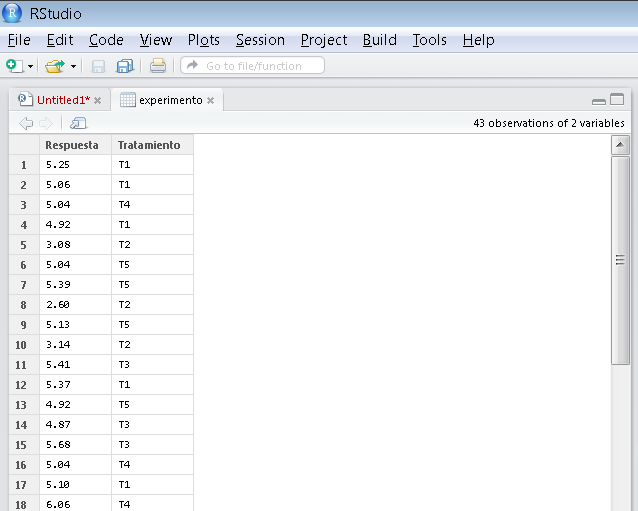
\includegraphics[width=12cm]{../fig/Tut08-05.png}
\end{center}

¿Cómo se usan los factores en R? La contestación no puede ser completa en el espacio de este tutorial, porque los factores son un ingrediente clave del lenguaje de R, e intervienen en muchísimas construcciones del sistema. Pero, en cualquier caso, podemos empezar por lo más sencillo. ¿Qué aspecto tiene un vector de tipo factor? En el caso del {\tt data.frame experimento} que acabamos de crear, al mostrar el vector \verb#experimento$Tratamiento# se obtiene esto:
\begin{knitrout}
\definecolor{shadecolor}{rgb}{0.969, 0.969, 0.969}\color{fgcolor}\begin{kframe}
\begin{alltt}
\hlstd{experimento}\hlopt{$}\hlstd{Tratamiento}
\end{alltt}
\begin{verbatim}
##  [1] T1 T1 T4 T1 T2 T5 T5 T2 T5 T2 T3 T1 T5 T3 T3 T4 T1 T4 T1 T5 T4 T3 T4
## [24] T4 T1 T4 T1 T2 T3 T5 T5 T4 T2 T4 T4 T5 T1 T3 T3 T1 T3 T2 T2
## Levels: T1 T2 T3 T4 T5
\end{verbatim}
\end{kframe}
\end{knitrout}

Como se ve, R muestra el contenido del vector, junto con sus niveles. Si sólo queremos mostrar los niveles del factor, podemos usar la función {\tt levels}, así:

\begin{knitrout}
\definecolor{shadecolor}{rgb}{0.969, 0.969, 0.969}\color{fgcolor}\begin{kframe}
\begin{alltt}
\hlkwd{levels}\hlstd{(experimento}\hlopt{$}\hlstd{Tratamiento)}
\end{alltt}
\begin{verbatim}
## [1] "T1" "T2" "T3" "T4" "T5"
\end{verbatim}
\end{kframe}
\end{knitrout}

Fíjate en que en el factor no aparecián comillas, pero que al usar {\tt levels} sí que  aparecen. ¿Qué diferencia hay entre las dos situaciones? Para entender esto, es preciso recordar que en R las comillas indican que estamos ante un vector de tipo character.

Para verlo más claramente podemos pedirle a R que convierta el {\tt factor} en {\tt character} mediante la función {\tt as.character}:
\begin{knitrout}
\definecolor{shadecolor}{rgb}{0.969, 0.969, 0.969}\color{fgcolor}\begin{kframe}
\begin{alltt}
\hlkwd{as.character}\hlstd{(experimento}\hlopt{$}\hlstd{Tratamiento)}
\end{alltt}
\begin{verbatim}
##  [1] "T1" "T1" "T4" "T1" "T2" "T5" "T5" "T2" "T5" "T2" "T3" "T1" "T5" "T3"
## [15] "T3" "T4" "T1" "T4" "T1" "T5" "T4" "T3" "T4" "T4" "T1" "T4" "T1" "T2"
## [29] "T3" "T5" "T5" "T4" "T2" "T4" "T4" "T5" "T1" "T3" "T3" "T1" "T3" "T2"
## [43] "T2"
\end{verbatim}
\end{kframe}
\end{knitrout}

Las comillas que aparecen en este caso indican precisamente que se trata de un vector de tipo {\tt character}. Los factores, en cambio, son otra cosa: aunque los factores representan variables cualitativas, R los gestiona internamente (de forma más eficiente) mediante códigos numéricos. Al mostrarlos, a petición nuestra, el uso de las comillas permite distinguir entre un vector de tipo {\tt character} (con comillas) y un vector de tipo {\tt factor} (sin comillas).

Cuando usamos {\tt levels} le estamos pidiendo a R que nos enseñe los {\em nombres} de los niveles del factor. Y, en tanto que nombres, estamos hablando de valores de tipo {\tt character}. Pero no hay que confundir el nivel con el {\em nombre del nivel}. Para tratar de aclararlo un poco más: si tienes un factor {\tt genero}, con muchos datos (imagínate miles de ellos), es posible que sus niveles se llamen {\tt hombre} y {\tt mujer}. Si un usuario de habla inglesa recibe ese fichero de datos, es probable que quiera cambiar {\em los nombres} de los niveles por {\tt man} y {\tt woman} respectivamente, pero ese cambio de nombre sólo afecta a dos {\em palabras} y no afecta en absoluto a la forma en la que R gestiona internamente los niveles (los miles de datos).


\subsubsection{Creando un factor manualmente.}

Como hemos dicho, cuando R usa una función como {\tt read.table} para cargar un {\tt data.frame}, los campos alfanuméricos (que contienen cadenas de texto, como el campo {\tt tratamientos} de nuestro ejemplo) se convierten, {\em por defecto} en factores. Pero puede que, a veces, queramos preservar esos datos como variables de tipo {\tt character}. Si es eso lo que queremos, basta con usar la opción {\tt stringsAsFactors=FALSE} en la función {\tt read.table}.

En cualquier caso, el uso de {\tt read.table} y funciones similares es la forma más habitual de ccrear factores en R. Pero en algunas ocasiones necesitaremos crear directamente un factor a partir de un vector de datos ya existente. La forma de hacerlo es usando la función {\tt factor}. Por ejemplo, antes hemos definido el vector

\begin{knitrout}
\definecolor{shadecolor}{rgb}{0.969, 0.969, 0.969}\color{fgcolor}\begin{kframe}
\begin{alltt}
\hlstd{pacientesPorGenero}
\end{alltt}
\begin{verbatim}
##  [1] "hombre" "mujer"  "mujer"  "hombre" "mujer"  "hombre" "hombre"
##  [8] "hombre" "mujer"  "mujer"  "mujer"
\end{verbatim}
\end{kframe}
\end{knitrout}

Este vector es de tipo {\tt character}. No es, por lo tanto, un factor (como indican las comillas).
Para crear un vector llamado {\tt genero}  de tipo {\tt factor} a partir de estos datos, usamos la función factor de la forma más  sencilla posible:

\begin{knitrout}
\definecolor{shadecolor}{rgb}{0.969, 0.969, 0.969}\color{fgcolor}\begin{kframe}
\begin{alltt}
\hlstd{(genero} \hlkwb{=} \hlkwd{factor}\hlstd{(pacientesPorGenero))}
\end{alltt}
\begin{verbatim}
##  [1] hombre mujer  mujer  hombre mujer  hombre hombre hombre mujer  mujer 
## [11] mujer 
## Levels: hombre mujer
\end{verbatim}
\end{kframe}
\end{knitrout}

Y ahora los niveles se obtienen con:
\begin{knitrout}
\definecolor{shadecolor}{rgb}{0.969, 0.969, 0.969}\color{fgcolor}\begin{kframe}
\begin{alltt}
\hlkwd{levels}\hlstd{(genero)}
\end{alltt}
\begin{verbatim}
## [1] "hombre" "mujer"
\end{verbatim}
\end{kframe}
\end{knitrout}

De hecho nuestro usuario angloparlante podría usar {\tt levels} para traducir los nombres de los niveles, así:

\begin{knitrout}
\definecolor{shadecolor}{rgb}{0.969, 0.969, 0.969}\color{fgcolor}\begin{kframe}
\begin{alltt}
\hlkwd{levels}\hlstd{(genero)} \hlkwb{=} \hlkwd{c}\hlstd{(}\hlstr{"man"}\hlstd{,} \hlstr{"woman"}\hlstd{)}
\hlstd{genero}
\end{alltt}
\begin{verbatim}
##  [1] man   woman woman man   woman man   man   man   woman woman woman
## Levels: man woman
\end{verbatim}
\end{kframe}
\end{knitrout}

Aunque también se puede aprovechar la creación del vector factor para cambiar los nombres de los niveles, usando la opción {\tt labels} de la función {\tt factor}:

\begin{knitrout}
\definecolor{shadecolor}{rgb}{0.969, 0.969, 0.969}\color{fgcolor}\begin{kframe}
\begin{alltt}
\hlstd{(genero} \hlkwb{=} \hlkwd{factor}\hlstd{(pacientesPorGenero,} \hlkwc{labels}\hlstd{=}\hlkwd{c}\hlstd{(}\hlstr{"man"}\hlstd{,} \hlstr{"woman"}\hlstd{)))}
\end{alltt}
\begin{verbatim}
##  [1] man   woman woman man   woman man   man   man   woman woman woman
## Levels: man woman
\end{verbatim}
\end{kframe}
\end{knitrout}

\subsubsection{Advertencia: sobre {\tt levels} y {\tt labels}.}

El matiz al que ahora nos vamos a referir resulta confuso para muchos usuarios principiantes de R. Así que si al principio te cuesta entenderlo, no te preocupes demasiado. Cuando tengas más experiencia y surja la necesidad de aclararlo, podrás volver sobre estas ideas. Intenta hacer una primera lectura de este apartado, pero si te pierdes, sigue adelante. Ya habrá tiempo más adelante para entenderlo bien.

El método que acabamos de presentar, usando {\tt labels} ha funcionado en este caso porque el orden alfabético de {\em hombre}, {\em mujer} en español coincide con el orden de {\em man}, {\em woman} en inglés. Pero imagínate que el vector original estuviera en alemán. En ese idioma {\em hombre} y {\em mujer} se dicen, respectivamente, {\em Mann} y {\em Frau}.  Así que, como ves, el orden alfabético es distinto. El vector original, en alemán, sería:

\begin{knitrout}
\definecolor{shadecolor}{rgb}{0.969, 0.969, 0.969}\color{fgcolor}\begin{kframe}
\begin{alltt}
\hlstd{pacientesPorGenero}\hlkwb{=}\hlkwd{c}\hlstd{(}\hlstr{"Mann"}\hlstd{,} \hlstr{"Frau"}\hlstd{,} \hlstr{"Frau"}\hlstd{,} \hlstr{"Mann"}\hlstd{,} \hlstr{"Frau"}\hlstd{,} \hlstr{"Mann"}\hlstd{,} \hlstr{"Mann"}\hlstd{,} \hlstr{"Mann"}\hlstd{,}
    \hlstr{"Frau"}\hlstd{,} \hlstr{"Frau"}\hlstd{,} \hlstr{"Frau"}\hlstd{)}
\end{alltt}
\end{kframe}
\end{knitrout}
Y si ahora le aplicas {\tt factor} directamente, como hemos hecho antes, se obtiene:

\begin{knitrout}
\definecolor{shadecolor}{rgb}{0.969, 0.969, 0.969}\color{fgcolor}\begin{kframe}
\begin{alltt}
\hlstd{(genero} \hlkwb{=} \hlkwd{factor}\hlstd{(pacientesPorGenero))}
\end{alltt}
\begin{verbatim}
##  [1] Mann Frau Frau Mann Frau Mann Mann Mann Frau Frau Frau
## Levels: Frau Mann
\end{verbatim}
\end{kframe}
\end{knitrout}


Lo más importante es que te fijes en que R escribe los factores {\bf en orden alfabético:} primero {\tt Frau} y luego {\tt Mann}. Y eso tiene una consecuencia muy importante. Si, ingenuamente, tratas de hacer la traducción al español:

\begin{knitrout}
\definecolor{shadecolor}{rgb}{0.969, 0.969, 0.969}\color{fgcolor}\begin{kframe}
\begin{alltt}
\hlstd{(genero} \hlkwb{=} \hlkwd{factor}\hlstd{(pacientesPorGenero,} \hlkwc{labels}\hlstd{=}\hlkwd{c}\hlstd{(}\hlstr{"hombre"}\hlstd{,} \hlstr{"mujer"}\hlstd{)))}
\end{alltt}
\begin{verbatim}
##  [1] mujer  hombre hombre mujer  hombre mujer  mujer  mujer  hombre hombre
## [11] hombre
## Levels: hombre mujer
\end{verbatim}
\end{kframe}
\end{knitrout}
enseguida descubrirás que hombres y mujeres se han intercambiado. ¿Cómo ha sucedido esto? Vamos despacio, para entender lo que ocurre y ver cómo evitarlo.


Para convertir el vector {\tt pacientesPorGenero} en un factor, lo primero que hace R es aplicarle la función {\tt unique}, para ver cuáles son las {\em palabras distintas} que aparecen en ese vector:

\begin{knitrout}
\definecolor{shadecolor}{rgb}{0.969, 0.969, 0.969}\color{fgcolor}\begin{kframe}
\begin{alltt}
\hlkwd{unique}\hlstd{(pacientesPorGenero)}
\end{alltt}
\begin{verbatim}
## [1] "Mann" "Frau"
\end{verbatim}
\end{kframe}
\end{knitrout}

Pero el resultado no está ordenado alfabéticamente, como queda patente en este ejemplo. Y ahora viene el paso clave: lo siguiente que hace R es ordenar alfabéticamente estas palabras, usando la función {\tt sort}:

\begin{knitrout}
\definecolor{shadecolor}{rgb}{0.969, 0.969, 0.969}\color{fgcolor}\begin{kframe}
\begin{alltt}
\hlkwd{sort}\hlstd{(}\hlkwd{unique}\hlstd{(pacientesPorGenero))}
\end{alltt}
\begin{verbatim}
## [1] "Frau" "Mann"
\end{verbatim}
\end{kframe}
\end{knitrout}

Esta lista {\em ordenada alfabéticamente} es la que R usa para establecer los niveles del factor {\em y el orden de sus etiquetas}. Así que cuando hemos usado {\tt labels} para traducir, R ha interpretado que {\em hombre} era la traducción de {\em Frau} (la primera etiqueta por orden alfabético) mientras que {\em mujer } es la traducción de {\em Mann}. Un pequeño desastre, pero que, en algunas ocasiones, le ha costado un disgusto a más de un usuario de R desprevenido.

¿Cómo lo arreglamos? Con un argumento opcional de {\tt factor}, llamado quizá confusamente {\tt levels},  que nos deja escribir explícitamente el orden en el que queremos que R coloque los nombres de los niveles del factor. En este ejemplo, la solución consiste en hacer:

\begin{knitrout}
\definecolor{shadecolor}{rgb}{0.969, 0.969, 0.969}\color{fgcolor}\begin{kframe}
\begin{alltt}
\hlstd{(genero} \hlkwb{=} \hlkwd{factor}\hlstd{(pacientesPorGenero,}
        \hlkwc{levels} \hlstd{=} \hlkwd{c}\hlstd{(}\hlstr{"Mann"}\hlstd{,} \hlstr{"Frau"}\hlstd{),} \hlkwc{labels}\hlstd{=}\hlkwd{c}\hlstd{(}\hlstr{"hombre"}\hlstd{,} \hlstr{"mujer"}\hlstd{)))}
\end{alltt}
\begin{verbatim}
##  [1] hombre mujer  mujer  hombre mujer  hombre hombre hombre mujer  mujer 
## [11] mujer 
## Levels: hombre mujer
\end{verbatim}
\end{kframe}
\end{knitrout}

Al trabajar de esta manera, nos aseguramos de que el orden de los términos en {\tt levels} coincide con el de {\tt labels} y evitamos cualquier riesgo de acabar confundidos, {\em lost in traslation}. Naturalmente, aunque hemos usado un ejemplo con distintos idiomas, esta situación puede presentarse con cualquier cambio en los niveles de un factor. Imagínate que estamos trabajando en gestión del tráfico por carretera y queremos crear un factor que indique el código correspondiente al estado del tráfico en distintas carreteras. Podríamos ser algo como:

\begin{knitrout}
\definecolor{shadecolor}{rgb}{0.969, 0.969, 0.969}\color{fgcolor}\begin{kframe}
\begin{alltt}
\hlstd{(estadoCarreteras} \hlkwb{=} \hlkwd{factor}\hlstd{(}\hlkwd{c}\hlstd{(}\hlstr{"rojo"}\hlstd{,} \hlstr{"verde"}\hlstd{,} \hlstr{"amarillo"}\hlstd{,} \hlstr{"verde"}\hlstd{,} \hlstr{"rojo"}\hlstd{,}
    \hlstr{"amarillo"}\hlstd{,} \hlstr{"verde"}\hlstd{,} \hlstr{"verde"}\hlstd{,} \hlstr{"rojo"}\hlstd{,} \hlstr{"amarillo"}\hlstd{)))}
\end{alltt}
\begin{verbatim}
##  [1] rojo     verde    amarillo verde    rojo     amarillo verde   
##  [8] verde    rojo     amarillo
## Levels: amarillo rojo verde
\end{verbatim}
\end{kframe}
\end{knitrout}

¿Te has fijado en el orden en el que R ha escrito los niveles? Es el orden alfabético, claro. Si quieres mantener un orden concreto como {\em rojo, amarillo, verde}, debes usar {\tt levels} y hacer algo como esto:

\begin{knitrout}
\definecolor{shadecolor}{rgb}{0.969, 0.969, 0.969}\color{fgcolor}\begin{kframe}
\begin{alltt}
\hlstd{(estadoCarreteras} \hlkwb{=} \hlkwd{factor}\hlstd{(}\hlkwd{c}\hlstd{(}\hlstr{"rojo"}\hlstd{,} \hlstr{"verde"}\hlstd{,} \hlstr{"amarillo"}\hlstd{,} \hlstr{"verde"}\hlstd{,} \hlstr{"rojo"}\hlstd{,}
    \hlstr{"amarillo"}\hlstd{,} \hlstr{"verde"}\hlstd{,} \hlstr{"verde"}\hlstd{,} \hlstr{"rojo"}\hlstd{,} \hlstr{"amarillo"}\hlstd{),}
    \hlkwc{levels} \hlstd{=} \hlkwd{c}\hlstd{(}\hlstr{"rojo"}\hlstd{,} \hlstr{"amarillo"}\hlstd{,} \hlstr{"verde"}\hlstd{)))}
\end{alltt}
\begin{verbatim}
##  [1] rojo     verde    amarillo verde    rojo     amarillo verde   
##  [8] verde    rojo     amarillo
## Levels: rojo amarillo verde
\end{verbatim}
\end{kframe}
\end{knitrout}

Y si además quieres usar {\tt labels} para cambiar las {\em etiquetas}, asegúrate de que mantienes el mismo orden:


\begin{knitrout}
\definecolor{shadecolor}{rgb}{0.969, 0.969, 0.969}\color{fgcolor}\begin{kframe}
\begin{alltt}
\hlstd{(estadoCarreteras} \hlkwb{=} \hlkwd{factor}\hlstd{(}\hlkwd{c}\hlstd{(}\hlstr{"rojo"}\hlstd{,} \hlstr{"verde"}\hlstd{,} \hlstr{"amarillo"}\hlstd{,} \hlstr{"verde"}\hlstd{,} \hlstr{"rojo"}\hlstd{,}
    \hlstr{"amarillo"}\hlstd{,} \hlstr{"verde"}\hlstd{,} \hlstr{"verde"}\hlstd{,} \hlstr{"rojo"}\hlstd{,} \hlstr{"amarillo"}\hlstd{),}
    \hlkwc{levels} \hlstd{=} \hlkwd{c}\hlstd{(}\hlstr{"rojo"}\hlstd{,} \hlstr{"amarillo"}\hlstd{,} \hlstr{"verde"}\hlstd{),}
    \hlkwc{labels} \hlstd{=} \hlkwd{c}\hlstd{(}\hlstr{"atasco"}\hlstd{,} \hlstr{"moderado"}\hlstd{,} \hlstr{"fluido"}\hlstd{)))}
\end{alltt}
\begin{verbatim}
##  [1] atasco   fluido   moderado fluido   atasco   moderado fluido  
##  [8] fluido   atasco   moderado
## Levels: atasco moderado fluido
\end{verbatim}
\end{kframe}
\end{knitrout}

Para terminar con esta cuestión tan espinosa de los niveles de un factor y sus etiquetas, vamos a suponer que has creado el factor, poniendo cuidado en elegir el orden de los niveles con {\tt levels}:

\begin{knitrout}
\definecolor{shadecolor}{rgb}{0.969, 0.969, 0.969}\color{fgcolor}\begin{kframe}
\begin{alltt}
\hlstd{(estadoCarreteras} \hlkwb{=} \hlkwd{factor}\hlstd{(}\hlkwd{c}\hlstd{(}\hlstr{"rojo"}\hlstd{,} \hlstr{"verde"}\hlstd{,} \hlstr{"amarillo"}\hlstd{,} \hlstr{"verde"}\hlstd{,} \hlstr{"rojo"}\hlstd{,}
    \hlstr{"amarillo"}\hlstd{,} \hlstr{"verde"}\hlstd{,} \hlstr{"verde"}\hlstd{,} \hlstr{"rojo"}\hlstd{,} \hlstr{"amarillo"}\hlstd{),}
    \hlkwc{levels} \hlstd{=} \hlkwd{c}\hlstd{(}\hlstr{"rojo"}\hlstd{,} \hlstr{"amarillo"}\hlstd{,} \hlstr{"verde"}\hlstd{)))}
\end{alltt}
\begin{verbatim}
##  [1] rojo     verde    amarillo verde    rojo     amarillo verde   
##  [8] verde    rojo     amarillo
## Levels: rojo amarillo verde
\end{verbatim}
\end{kframe}
\end{knitrout}

y que {\em a posteriori} decides cambiar {\em los nombres} de las etiquetas. Por ejemplo, vamos a cambiar
{\em rojo, amarillo, verde} por {\em atasco, moderado, fluido}. Para hacer esto, usamos la función {\tt levels} de nuevo:
\begin{knitrout}
\definecolor{shadecolor}{rgb}{0.969, 0.969, 0.969}\color{fgcolor}\begin{kframe}
\begin{alltt}
\hlkwd{levels}\hlstd{(estadoCarreteras)} \hlkwb{=} \hlkwd{c}\hlstd{(}\hlstr{"atasco"}\hlstd{,} \hlstr{"moderado"}\hlstd{,} \hlstr{"fluido"}\hlstd{)}
\hlstd{estadoCarreteras}
\end{alltt}
\begin{verbatim}
##  [1] atasco   fluido   moderado fluido   atasco   moderado fluido  
##  [8] fluido   atasco   moderado
## Levels: atasco moderado fluido
\end{verbatim}
\end{kframe}
\end{knitrout}
Personalmente, encuentro este último punto especialmente confuso y en su momento me costó trabajo asimilarlo. Fíjate en que antes, cuando lo hacíamos durante la creación del factor usábamos {\tt labels} pero ahora, a posteriori, debemos usar {\tt levels}. De hecho, si tratas de usar {\tt labels} para esto ¡R se enfada!:
\begin{knitrout}
\definecolor{shadecolor}{rgb}{0.969, 0.969, 0.969}\color{fgcolor}\begin{kframe}
\begin{alltt}
\hlkwd{labels}\hlstd{(estadoCarreteras)} \hlkwb{=} \hlkwd{c}\hlstd{(}\hlstr{"atasco"}\hlstd{,} \hlstr{"moderado"}\hlstd{,} \hlstr{"fluido"}\hlstd{)}
\end{alltt}


{\ttfamily\noindent\bfseries\color{errorcolor}{\#\# Error in labels(estadoCarreteras) = c("{}atasco"{}, "{}moderado"{}, "{}fluido"{}): no se pudo encontrar la funci'on "{}labels<-"{}}}\end{kframe}
\end{knitrout}
Como hemos dicho, todo este pequeño lío de {\tt levels} y {\tt labels} te costará algo de trabajo al principio (y no es, desde luego, uno de los aspectos mejor resueltos de R) pero con la experiencia irás comprendiéndolo mejor.


\subsection{Usando los factores para explorar los datos}
\label{tut08:sec:UsandoFactoresExplorarDatos}

Los factores permiten modular el comportamiento de algunas funciones de R, de manera que la información que se obtiene tiene en cuenta esa organización en niveles de los valores que estamos analizando. Por ejemplo, en  el Tutorial02 vimos como usar la función {\tt summary} de R para obtener un resumen descriptivo de un vector de datos (media y percentiles, básicamente). Ahora, que tenemos un {\tt data.frame} con una clasificación por tratamientos, nos gustaría seguramente obtener esa misma información, pero para cada uno de los distintos tratamientos por separado. Lo primero que queremos hacer notar es que no sirve aplicar {\tt summary} directamente al {\tt data.frame}:

\begin{knitrout}
\definecolor{shadecolor}{rgb}{0.969, 0.969, 0.969}\color{fgcolor}\begin{kframe}
\begin{alltt}
\hlkwd{summary}\hlstd{(experimento)}
\end{alltt}
\begin{verbatim}
##    Respuesta    Tratamiento
##  Min.   :2.60   T1:10      
##  1st Qu.:4.54   T2: 7      
##  Median :5.04   T3: 8      
##  Mean   :4.79   T4:10      
##  3rd Qu.:5.25   T5: 8      
##  Max.   :6.06
\end{verbatim}
\end{kframe}
\end{knitrout}

Como se ve, se obtiene un resumen por separado para cada uno de los campos del {\tt data.frame},  con {\tt Respuesta} por un lado, y {\tt Tratamiento} por otro, sin reconocer el vínculo entre ambas. Naturalmente, puesto que ya hemos aprendido a seleccionar los elementos de un vector mediante condiciones (usando los corchetes {\tt [ ]}), podemos ir separando cada uno de los grupos de tratamiento, y aplicarles la función {\tt summary} a los vectores resultantes. Sería algo como esto (mostramos, por ejemplo el segundo grupo de tratamiento):
\begin{knitrout}
\definecolor{shadecolor}{rgb}{0.969, 0.969, 0.969}\color{fgcolor}\begin{kframe}
\begin{alltt}
\hlstd{(tratamiento2} \hlkwb{=} \hlstd{experimento[experimento}\hlopt{$}\hlstd{Tratamiento} \hlopt{==} \hlstr{"T2"}\hlstd{,} \hlnum{1}\hlstd{])}
\end{alltt}
\begin{verbatim}
## [1] 3.08 2.60 3.14 3.36 3.31 3.83 3.18
\end{verbatim}
\begin{alltt}
\hlkwd{summary}\hlstd{(tratamiento2)}
\end{alltt}
\begin{verbatim}
##    Min. 1st Qu.  Median    Mean 3rd Qu.    Max. 
##    2.60    3.11    3.18    3.21    3.33    3.83
\end{verbatim}
\end{kframe}
\end{knitrout}

Esto funciona, pero como se puede apreciar, trabajar así es engorroso. Para obtener lo que queremos, hay una manera mucho más natural de proceder, usando la función {\tt tapply}. Veamos como funciona:
%  (primero hemos usado {\tt attach} para poder referirnos a las variables {\tt Respuesta} y {\tt Tratamiento} sin tener que usar el \verb#$#)

\begin{knitrout}
\definecolor{shadecolor}{rgb}{0.969, 0.969, 0.969}\color{fgcolor}\begin{kframe}
\begin{alltt}
\hlkwd{tapply}\hlstd{(experimento}\hlopt{$}\hlstd{Respuesta, experimento}\hlopt{$}\hlstd{Tratamiento, summary)}
\end{alltt}
\begin{verbatim}
## $T1
##    Min. 1st Qu.  Median    Mean 3rd Qu.    Max. 
##    4.70    4.96    5.08    5.08    5.23    5.37 
## 
## $T2
##    Min. 1st Qu.  Median    Mean 3rd Qu.    Max. 
##    2.60    3.11    3.18    3.21    3.33    3.83 
## 
## $T3
##    Min. 1st Qu.  Median    Mean 3rd Qu.    Max. 
##    4.52    5.01    5.29    5.23    5.48    5.71 
## 
## $T4
##    Min. 1st Qu.  Median    Mean 3rd Qu.    Max. 
##    4.40    4.61    4.97    5.06    5.40    6.06 
## 
## $T5
##    Min. 1st Qu.  Median    Mean 3rd Qu.    Max. 
##    4.56    4.93    5.01    5.04    5.18    5.39
\end{verbatim}
\end{kframe}
\end{knitrout}

Ahora sí: como ves, R ha reconocido esa estructura en niveles del factor {\tt Tratamiento}, y no está describiendo la variable {\tt Respuesta} para cada uno de los grupos de tratamiento que conforman nuestros datos. El resultado es una {\em tabla} (de ahí la {\tt t} inicial de {\tt tapply}) que contiene, ordenados por filas, los resultados de aplicar la función {\tt summary} a los valores de {\tt Respuesta}, agrupadas según los distintos niveles del factor {\tt Tratamiento}.

Otro ejemplo de las ventajas del lenguaje de factores se obtiene al pensar en la función {\tt boxplot}. Si aplicamos esa función directamente al {\tt data.frame}, ejecutando:
\begin{knitrout}
\definecolor{shadecolor}{rgb}{0.969, 0.969, 0.969}\color{fgcolor}\begin{kframe}
\begin{alltt}
\hlkwd{boxplot}\hlstd{(experimento)}
\end{alltt}
\end{kframe}
\includegraphics[width=\maxwidth]{figure/unnamed-chunk-52-1} 

\end{knitrout}
se obtiene un gráfico que es, de hecho un sinsentido. Fíjate en que se incluye un boxplot para la variable {\tt Tratamiento} ¡qué es cualitativa! Evidentemente esto no es correcto. Para obtener lo que queremos basta con escribir:

\begin{knitrout}
\definecolor{shadecolor}{rgb}{0.969, 0.969, 0.969}\color{fgcolor}\begin{kframe}
\begin{alltt}
\hlkwd{boxplot}\hlstd{(Respuesta} \hlopt{~} \hlstd{Tratamiento,} \hlkwc{data} \hlstd{= experimento)}
\end{alltt}
\end{kframe}
\includegraphics[width=\maxwidth]{figure/unnamed-chunk-53-1} 

\end{knitrout}

El resultado es un gráfico mucho más adecuado para comparar los resultados de los tratamientos.

La sintaxis \verb#Respuesta ~ Tratamiento# que hemos usado por primera vez en esta llamada, es la que usa R para decir algo así como {\em ``la forma en que los valores de {\tt Respuesta} dependen de los tratamientos''}. Este tipo de expresiones se denominan {\sf fórmulas} en R. Y en general, en R, el símbolo \verb#~# se utiliza para indicar una dependencia o relación entre variables (lo obtienes, en un teclado estándar de PC, pulsando las teclas {\tt AltGr} y $4$ a la vez). En este caso, lo que estamos estudiando es si hay alguna relación entre la variable cualitativa (factor) {\tt Tratamiento}, y la variable cuantitativa {\tt Respuesta}. En particular, una pregunta que a menudo nos interesa consiste en saber si la respuesta media al tratamiento es distinta según el grupo de tratamiento que se considere.  Este tipo de problemas, en los que se investiga la relación entre varias variables aleatorias (de distintos tipos), forman el contenido de la cuarta parte del curso, y por eso estamos empezando a preparar el terreno en este tutorial.

\subsection{La función {\tt cut}}

Otra de las primeras funciones de R que se aprenden al comenzar a trabajar con factores es la función {\tt cut}, cortar en inglés. Y el nombre describe muy bien lo que hace esta función. Se usa para cortar en piezas los datos de  una variable cuantitativa, con el fin de agruparlos en clases o intervalos, como discutimos en la Sección \ref{curso-cap01:subsec:NotacionVariablesTablasFrecuenciaDatosAgrupados} del Capítulo \ref{curso-cap:IntroduccionEstadisticaDescriptiva} del libro.

Por ejemplo, el fichero adjunto
\begin{center}
\fichero{../datos/Tut08-Edades.csv}{Tut08-Edades.csv}
\end{center}
contiene las edades, en años, de un grupo de $500$ personas. Imagínate que queremos agrupar esos datos, según la edad, en estas categorías:

\begin{itemize}
  \item {\em Menores}, con edades menores que 18 años,
  \item {\em Jovenes}, con edades entre 18 y 30 años,
  \item {\em MedianaEdad}, con edades entre 31 y 64 años,
  \item {\em Mayores}, con edades de 65 años en adelante.
\end{itemize}
Vamos a ver como usar {\tt cut} para hacer eso en R. Primero leemos el fichero (recuerda que debe estar en la carpeta {\tt datos} del {\em Directorio de Trabajo}) y lo guardamos en un vector de datos, llamado {\tt edades}, al que aplicaremos la función {\tt cut}.

\begin{knitrout}
\definecolor{shadecolor}{rgb}{0.969, 0.969, 0.969}\color{fgcolor}\begin{kframe}
\begin{alltt}
\hlstd{edades} \hlkwb{=} \hlkwd{read.table}\hlstd{(}\hlkwc{file}\hlstd{=}\hlstr{"../datos/Tut08-Edades.csv"}\hlstd{)[ ,}\hlnum{1}\hlstd{]}
\end{alltt}
\end{kframe}
\end{knitrout}

Pero antes de cortar, tenemos que pensar bien dónde vamos a dar los cortes. Los intervalos que R usa, en la función {\tt cut} son, por defecto, de la forma $(a,b]$. Es decir, incluyen el límite derecho pero no el izquierdo (esto se puede cambiar). Eso implica que so hacemos una elección poco cuidadosa de los puntos de corte, como en:
\begin{knitrout}
\definecolor{shadecolor}{rgb}{0.969, 0.969, 0.969}\color{fgcolor}\begin{kframe}
\begin{alltt}
\hlstd{cortesEdad} \hlkwb{=} \hlkwd{c}\hlstd{(}\hlnum{0}\hlstd{,} \hlnum{18}\hlstd{,} \hlnum{30}\hlstd{,} \hlnum{65}\hlstd{,} \hlnum{100}\hlstd{)}
\end{alltt}
\end{kframe}
\end{knitrout}
terminaremos con un intervalo de edades como $18< edad \leq 30$, que no se corresponde con lo que queremos, porque no incluye a las personas de 18 años. Algo parecido sucede con el intervalo $30 < edad \leq 65$, que no es lo que queremos porque incluye a las personas de 65 años. Una elección algo más meditada nos conduce a:
\begin{knitrout}
\definecolor{shadecolor}{rgb}{0.969, 0.969, 0.969}\color{fgcolor}\begin{kframe}
\begin{alltt}
\hlstd{cortesEdad} \hlkwb{=} \hlkwd{c}\hlstd{(}\hlnum{0}\hlstd{,} \hlnum{17}\hlstd{,} \hlnum{30}\hlstd{,} \hlnum{64}\hlstd{,} \hlnum{100}\hlstd{)}
\end{alltt}
\end{kframe}
\end{knitrout}
Esto está casi bien, pero aún tenemos un problema. ¿Cuáles son los intervalos $(a,b]$ determinados por este segundo vector {\tt cortesEdad}? El primer intervalo es $(0,17]$. Eso significa que si alguna de las edades es $0$ (como, de hecho, sucede), no quedará incluida en ese intervalo. Para evitar ese problema, la función {\tt cut} dispone de una opción, {\tt include.lowest=TRUE}, que permite cerrar a la izquierda el primero de los intervalos. Con eso estamos listos para usar la función {\tt cut}:

\begin{knitrout}
\definecolor{shadecolor}{rgb}{0.969, 0.969, 0.969}\color{fgcolor}\begin{kframe}
\begin{alltt}
\hlstd{factorEdad} \hlkwb{=} \hlkwd{cut}\hlstd{(edades,} \hlkwc{breaks}\hlstd{=cortesEdad,} \hlkwc{include.lowest}\hlstd{=}\hlnum{TRUE}\hlstd{)}
\end{alltt}
\end{kframe}
\end{knitrout}

El resultado, que hemos guardado en la variable {\tt factorEdad} es un vector, de tipo {\tt factor} (puedes usar {\tt class(factorEdad)} para comprobarlo), que contiene, para cada elemento de {\tt edades} el intervalo de edades (nivel del factor) al que pertenece. Para que lo veas con más claridad, vamos a ver, juntos, los primeros elementos de los vectores {\tt edades} y {\tt factorEdad}, usando {\tt head}:

\begin{knitrout}
\definecolor{shadecolor}{rgb}{0.969, 0.969, 0.969}\color{fgcolor}\begin{kframe}
\begin{alltt}
\hlkwd{head}\hlstd{(edades)}
\end{alltt}
\begin{verbatim}
## [1] 16 59 27 32 45 59
\end{verbatim}
\begin{alltt}
\hlkwd{head}\hlstd{(factorEdad)}
\end{alltt}
\begin{verbatim}
## [1] [0,17]  (30,64] (17,30] (30,64] (30,64] (30,64]
## Levels: [0,17] (17,30] (30,64] (64,100]
\end{verbatim}
\end{kframe}
\end{knitrout}

Como ves, en cada posición de {\tt factorEdad} está el intervalo de edades (nivel del factor) al que pertenece el correspondiente elemento de {\tt edades}. Fíjate en que el intervalo del primer elemento es  [0,17] %{\tt [0,17]}
, cerrado en ambos extremos.

Además, R nos  recuerda al final el conjunto de nombres de los valores (niveles) que puede tomar el factor. Como hemos visto, los niveles de un factor se pueden obtener (y modificar) usando la función {\tt levels} así:
\begin{knitrout}
\definecolor{shadecolor}{rgb}{0.969, 0.969, 0.969}\color{fgcolor}\begin{kframe}
\begin{alltt}
\hlkwd{levels}\hlstd{(factorEdad)}
\end{alltt}
\begin{verbatim}
## [1] "[0,17]"   "(17,30]"  "(30,64]"  "(64,100]"
\end{verbatim}
\end{kframe}
\end{knitrout}
Insistimos en que estos son {\em los nombres de los niveles}, para recordar que, internamente, R utiliza códigos numéricos para trabajar con los niveles. Por eso es bueno usar una palabra como {\sf etiquetas} para referirse a esos nombres.

Y, como hemos visto,  si queremos cambiar estas etiquetas, podemos reemplazarlas con otras más útiles para nosotros. La forma de hacerlo, en este ejemplo, es esta:
\begin{knitrout}
\definecolor{shadecolor}{rgb}{0.969, 0.969, 0.969}\color{fgcolor}\begin{kframe}
\begin{alltt}
\hlkwd{levels}\hlstd{(factorEdad)} \hlkwb{=} \hlkwd{c}\hlstd{(}\hlstr{"menor"}\hlstd{,} \hlstr{"joven"}\hlstd{,} \hlstr{"medianaEdad"}\hlstd{,} \hlstr{"mayor"}\hlstd{)}
\end{alltt}
\end{kframe}
\end{knitrout}

Ahora, si pruebas a ejecutar de nuevo {\tt head(factorEdad)}, verás el efecto que ha tenido ese cambio. %Para lo que resta de trabajo, vamos a devolver al factor a sus etiquetas iniciales, que son más concisas:
%<<>>=
%levels(factorEdad)=c("[0,17]",   "(17,30]",  "(30,64]",  "(64,100]")
%@
%Podemos, con ayuda del factor, obtener muy fácilmente una tabla de frecuencias de las edades (se muestra la salida):
%<<>>=
%table(factorEdad)
%@
%y los resúmenes ({\tt summary}) o boxplots por niveles, etc., que ya hemos visto antes.



\section{Ejercicios adicionales y soluciones.}
\label{tut08:sec:EjerciciosAdicionalesYSoluciones}

%\subsection*{Ejercicios adicionales.}
%\label{tut08:subsec:EjerciciosAdicionales}
%
%\begin{ejercicio}
%\label{tut08:ejercicio26}
%
%\qed
%\end{ejercicio}
%

%%##########################################

\subsection*{Soluciones de algunos ejercicios.}
\label{tut08:subsec:SolucionesAlgunosEjercicios}


\paragraph{\bf $\bullet$ Ejercicio \ref{tut08:ejercicio01}, pág. \pageref{tut08:ejercicio01}}
\label{tut08:ejercicio01:sol}\quad\\

\begin{enumerate}
  \item Incluimos aquí el código del fichero con los datos de este ejercicio y el resultado que se obtiene.

\begin{knitrout}
\definecolor{shadecolor}{rgb}{0.969, 0.969, 0.969}\color{fgcolor}\begin{kframe}
\begin{alltt}
\hlcom{####################################################}
\hlcom{# www.postdata-statistics.com}
\hlcom{# POSTDATA. Introducci<U+00F3>n a la Estad<U+00ED>sitica}
\hlcom{# Tutorial-08.}
\hlcom{#}
\hlcom{# Fichero de instrucciones R para calcular}
\hlcom{# un intervalo de confianza (1-alfa) para la proporcion p de}
\hlcom{# una poblacion tipo Binomial (Bernouilli), a partir de una}
\hlcom{# muestra con n datos.}
\hlcom{#}
\hlcom{# Este fichero usa los valores de una muestra,}
\hlcom{# previamente calculados (numero de datos, proporcion muestral)}
\hlcom{#}
\hlcom{##############################################################}

\hlkwd{rm}\hlstd{(}\hlkwc{list}\hlstd{=}\hlkwd{ls}\hlstd{())} \hlcom{#limpieza inicial}

\hlcom{# Introduce el numero de datos de la muestra:}

\hlstd{n} \hlkwb{=} \hlnum{456}

\hlcom{# Introduce aqui el valor de pMuestral, la proporcion muestral .}
\hlcom{# Recuerda que pMuestral es el numero de casos favorables en la muestra}
\hlcom{# dividido por n.}

\hlstd{pMuestral} \hlkwb{=} \hlnum{139} \hlopt{/} \hlnum{456}

\hlcom{# LEE ESTAS INSTRUCCIONES ATENTAMENTE:}
\hlcom{# SI LA MUESTRA TIENE < 30 ELEMENTOS O SI N*p<5 O SI n*q<5,}
\hlcom{# NO USES ESTE FICHERO!!}
\hlcom{# ASEGURATE DE HABER ENTENDIDO ESTAS INSTRUCCIONES}

\hlcom{# Nivel de confianza deseado.}

\hlstd{nc} \hlkwb{=} \hlnum{0.95}

\hlcom{################################################}
\hlcom{#NO CAMBIES NADA DE AQUI PARA ABAJO}
\hlcom{################################################}
\hlstd{(alfa} \hlkwb{=} \hlnum{1} \hlopt{-} \hlstd{nc )}
\end{alltt}
\begin{verbatim}
## [1] 0.05
\end{verbatim}
\begin{alltt}
\hlcom{# Calculamos el valor critico:}

\hlstd{(z_alfa2} \hlkwb{=} \hlkwd{qnorm}\hlstd{(} \hlnum{1} \hlopt{-} \hlstd{alfa} \hlopt{/} \hlnum{2} \hlstd{) )}
\end{alltt}
\begin{verbatim}
## [1] 1.96
\end{verbatim}
\begin{alltt}
\hlcom{# Calculamos qMuestral}

\hlstd{qMuestral} \hlkwb{=} \hlnum{1} \hlopt{-} \hlstd{pMuestral}

\hlcom{# Comprobamos la condicion sobre n}
\hlkwa{if}\hlstd{((n}\hlopt{<=}\hlnum{30}\hlstd{)}\hlopt{|}\hlstd{(n}\hlopt{*}\hlstd{pMuestral}\hlopt{<}\hlnum{5}\hlstd{)}\hlopt{|}\hlstd{(n}\hlopt{*}\hlstd{qMuestral}\hlopt{<}\hlnum{5}\hlstd{))\{}
  \hlkwd{warning}\hlstd{(}\hlstr{"NO SE CUMPLEN LAS CONDICIONES"}\hlstd{)}
\hlstd{\}}


\hlcom{# Semianchura del intervalo}
\hlstd{(semianchura}\hlkwb{=}\hlstd{z_alfa2} \hlopt{*} \hlkwd{sqrt}\hlstd{(pMuestral} \hlopt{*} \hlstd{qMuestral} \hlopt{/} \hlstd{n) )}
\end{alltt}
\begin{verbatim}
## [1] 0.042251
\end{verbatim}
\begin{alltt}
\hlcom{# Y el intervalo de confianza (a,b) para mu es este:}

\hlstd{(intervalo} \hlkwb{=} \hlstd{pMuestral} \hlopt{+} \hlkwd{c}\hlstd{(}\hlopt{-}\hlnum{1}\hlstd{,} \hlnum{1}\hlstd{)} \hlopt{*} \hlstd{semianchura )}
\end{alltt}
\begin{verbatim}
## [1] 0.26257 0.34708
\end{verbatim}
\end{kframe}
\end{knitrout}

  \item Con {\tt prop.test} el intervalo se obtiene así:
\begin{knitrout}
\definecolor{shadecolor}{rgb}{0.969, 0.969, 0.969}\color{fgcolor}\begin{kframe}
\begin{alltt}
  \hlkwd{prop.test}\hlstd{(}\hlkwc{x} \hlstd{=} \hlnum{139}\hlstd{,} \hlkwc{n} \hlstd{=} \hlnum{456}\hlstd{,} \hlkwc{alternative} \hlstd{=} \hlstr{"two.sided"}\hlstd{,} \hlkwc{conf.level} \hlstd{=} \hlnum{0.95}\hlstd{)}
\end{alltt}
\begin{verbatim}
## 
## 	1-sample proportions test with continuity correction
## 
## data:  139 out of 456, null probability 0.5
## X-squared = 68.7, df = 1, p-value <2e-16
## alternative hypothesis: true p is not equal to 0.5
## 95 percent confidence interval:
##  0.26330 0.34969
## sample estimates:
##       p 
## 0.30482
\end{verbatim}
\end{kframe}
\end{knitrout}
  La función {\tt prop.test} también incluye un argumento {\tt p} que es lo que nosotros llamamos $p_0$ en el contraste de hipótesis. Para este ejercicio, dado que sólo estamos interesados en el intervalo de confianza, no es necesario incluir el valor de $p$.

  Para los datos de $2008$ es:
\begin{knitrout}
\definecolor{shadecolor}{rgb}{0.969, 0.969, 0.969}\color{fgcolor}\begin{kframe}
\begin{alltt}
  \hlkwd{prop.test}\hlstd{(}\hlkwc{x} \hlstd{=} \hlnum{138}\hlstd{,} \hlkwc{n} \hlstd{= (}\hlnum{138} \hlopt{+} \hlnum{270}\hlstd{),} \hlkwc{alternative} \hlstd{=} \hlstr{"two.sided"}\hlstd{,} \hlkwc{conf.level} \hlstd{=} \hlnum{0.95}\hlstd{)}
\end{alltt}
\begin{verbatim}
## 
## 	1-sample proportions test with continuity correction
## 
## data:  138 out of (138 + 270), null probability 0.5
## X-squared = 42.1, df = 1, p-value = 8.8e-11
## alternative hypothesis: true p is not equal to 0.5
## 95 percent confidence interval:
##  0.29285 0.38672
## sample estimates:
##       p 
## 0.33824
\end{verbatim}
\end{kframe}
\end{knitrout}

  \item En el panel de {\em Cálculo Simbólico} de GeoGebra o en la {\em Línea de Entrada} puedes usar este comando:
  \begin{verbatim}
    IntervaloProporciónZ[139/456, 456, 0.95]
  \end{verbatim}
  Recuerda ajustar el número de cifras en el menú opciones y recuerda también que la salida aparece en sitios distintos según utilices una u otra forma de entrada.

  También tienes la opción de usar la {\em Calculadora de Probabilidades} como se muestra en la figura:
    \begin{center}
    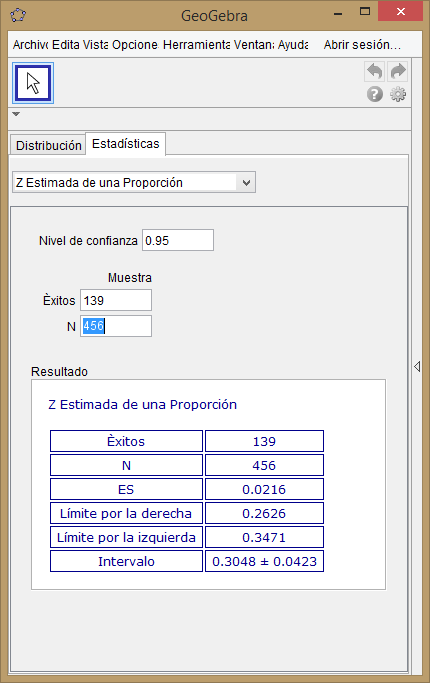
\includegraphics[width=8cm]{../fig/Tut08-08.png}
    \end{center}

\end{enumerate}

\paragraph{\bf $\bullet$ Ejercicio \ref{tut08:ejercicio02}, pág. \pageref{tut08:ejercicio02}}
\label{tut08:ejercicio02:sol}\quad\\

\begin{enumerate}

  \item Código del fichero con los datos de este ejercicio y el resultado que se obtiene:

        {\small
\begin{knitrout}
\definecolor{shadecolor}{rgb}{0.969, 0.969, 0.969}\color{fgcolor}\begin{kframe}
\begin{alltt}
\hlcom{####################################################}
\hlcom{# www.postdata-statistics.com}
\hlcom{# POSTDATA. Introducci<U+00F3>n a la Estad<U+00ED>sitica}
\hlcom{# Tutorial-08.}
\hlcom{#}
\hlcom{# Fichero de instrucciones R para calcular un contraste de}
\hlcom{# hipotesis para la proporcion, a partir de una}
\hlcom{#}
\hlcom{#         MUESTRA GRANDE}
\hlcom{#}
\hlcom{# con n >> 30 datos.}
\hlcom{#}
\hlcom{# El fichero no funcionara si no introduces todos los datos.}
\hlcom{#}
\hlcom{################################################################}

    \hlkwd{rm}\hlstd{(}\hlkwc{list}\hlstd{=}\hlkwd{ls}\hlstd{())}
\hlcom{# Numero de elementos en la muestra}
    \hlstd{(n}\hlkwb{=} \hlnum{105}\hlstd{)} \hlcom{#SE SUPONE QUE LA MUESTRA ES GRANDE, n>30}
\end{alltt}
\begin{verbatim}
## [1] 105
\end{verbatim}
\begin{alltt}
\hlcom{# Proporcion muestral (<U+00A1>es una fraccion! Numero de exitos/n)}
    \hlstd{(pMuestral}\hlkwb{=} \hlnum{39} \hlopt{/} \hlnum{105}\hlstd{)}
\end{alltt}
\begin{verbatim}
## [1] 0.37143
\end{verbatim}
\begin{alltt}
\hlcom{# Valor a contrastar de la proporcion (aparece en la hipotesis nula)}
    \hlstd{(p0}\hlkwb{=} \hlnum{0.35}\hlstd{)}
\end{alltt}
\begin{verbatim}
## [1] 0.35
\end{verbatim}
\begin{alltt}
\hlcom{# <U+00BF>Que tipo de contraste estamos haciendo?}
    \hlcom{# Escribe 1 si la HIP. ALTERNATIVA es p > p0, 2 si es p < p0, 3 si es p distinto de p0}
    \hlstd{TipoContraste} \hlkwb{=} \hlnum{1}
\hlcom{#Nivel de significacion}
    \hlstd{(nSig}\hlkwb{=} \hlnum{0.95}\hlstd{)}
\end{alltt}
\begin{verbatim}
## [1] 0.95
\end{verbatim}
\begin{alltt}
\hlcom{###############################################}
\hlcom{# NO CAMBIES NADA DE AQU<U+00CD> PARA ABAJO}
\hlcom{###############################################}

\hlcom{# Calculo de alfa}
    \hlstd{(alfa}\hlkwb{=}\hlnum{1}\hlopt{-}\hlstd{nSig)}
\end{alltt}
\begin{verbatim}
## [1] 0.05
\end{verbatim}
\begin{alltt}
\hlcom{# Calculo de q0}
    \hlstd{q0} \hlkwb{=} \hlnum{1}\hlopt{-} \hlstd{p0}
\hlcom{# Comprobamos la condicion sobre n}
\hlkwa{if}\hlstd{((n}\hlopt{<=}\hlnum{30}\hlstd{)}\hlopt{|}\hlstd{(n}\hlopt{*}\hlstd{p0}\hlopt{<}\hlnum{5}\hlstd{)}\hlopt{|}\hlstd{(n}\hlopt{*}\hlstd{q0}\hlopt{<}\hlnum{5}\hlstd{))\{}
  \hlkwd{warning}\hlstd{(}\hlstr{"NO SE CUMPLEN LAS CONDICIONES"}\hlstd{)}
\hlstd{\}}
\hlcom{# Calculo del estadistico del contraste}
    \hlstd{(Estadistico}\hlkwb{=}\hlstd{(pMuestral}\hlopt{-}\hlstd{p0)} \hlopt{/} \hlkwd{sqrt}\hlstd{( (p0} \hlopt{*} \hlstd{q0)} \hlopt{/} \hlstd{n ))}
\end{alltt}
\begin{verbatim}
## [1] 0.46036
\end{verbatim}
\begin{alltt}
\hlcom{# Funcion para el calculo del p-valor}
    \hlstd{pValor}\hlkwb{=}\hlkwa{function}\hlstd{(}\hlkwc{EstadCon}\hlstd{,}\hlkwc{tipoCon}\hlstd{)\{}
      \hlkwa{if}\hlstd{(tipoCon}\hlopt{==}\hlnum{1}\hlstd{)\{}
        \hlstd{(pV}\hlkwb{=}\hlnum{1}\hlopt{-}\hlkwd{pnorm}\hlstd{(EstadCon))}
      \hlstd{\}}
      \hlkwa{if}\hlstd{(tipoCon}\hlopt{==}\hlnum{2}\hlstd{)\{}
        \hlstd{(pV}\hlkwb{=}\hlkwd{pnorm}\hlstd{(EstadCon))}
      \hlstd{\}}
      \hlkwa{if}\hlstd{(tipoCon}\hlopt{==}\hlnum{3}\hlstd{)\{}
        \hlstd{pV}\hlkwb{=}\hlnum{2}\hlopt{*}\hlstd{(}\hlnum{1}\hlopt{-}\hlkwd{pnorm}\hlstd{(}\hlkwd{abs}\hlstd{(EstadCon)))}
      \hlstd{\}}
      \hlkwd{return}\hlstd{(}\hlkwd{paste}\hlstd{(}\hlstr{"El p-Valor es "}\hlstd{,pV,}\hlkwc{sep}\hlstd{=}\hlstr{""}\hlstd{,}\hlkwc{collapse}\hlstd{=}\hlstr{""}\hlstd{))}
    \hlstd{\}}
\hlcom{# Funcion para el calculo del l<U+00ED>mite de la regi<U+00F3>n de rechazo}
    \hlstd{RegionRechazo}\hlkwb{=}\hlkwa{function}\hlstd{(}\hlkwc{alfa}\hlstd{,}\hlkwc{tipoCon}\hlstd{)\{}
      \hlkwa{if}\hlstd{(tipoCon}\hlopt{==}\hlnum{1}\hlstd{)\{}
        \hlstd{(regionRech}\hlkwb{=}\hlkwd{paste}\hlstd{(}\hlstr{"valores del Estadistico mayores que "}\hlstd{,}\hlkwd{qnorm}\hlstd{(}\hlnum{1}\hlopt{-}\hlstd{alfa)) )}
      \hlstd{\}}
      \hlkwa{if}\hlstd{(tipoCon}\hlopt{==}\hlnum{2}\hlstd{)\{}
        \hlstd{(regionRech}\hlkwb{=}\hlkwd{paste}\hlstd{(}\hlstr{"valores del Estadistico menores que "}\hlstd{,}\hlkwd{qnorm}\hlstd{(alfa)) )}
      \hlstd{\}}
      \hlkwa{if}\hlstd{(tipoCon}\hlopt{==}\hlnum{3}\hlstd{)\{}
        \hlstd{(regionRech}\hlkwb{=}\hlkwd{paste}\hlstd{(}\hlstr{"valores del Estadistico mas alejados del origen que "}\hlstd{,}\hlkwd{qnorm}\hlstd{(}\hlnum{1}\hlopt{-}\hlstd{alfa}\hlopt{/}\hlnum{2}\hlstd{)) )}
      \hlstd{\}}
      \hlstd{regionRech}\hlkwb{=}\hlkwd{paste}\hlstd{(}\hlstr{"La region de rechazo la forman los "}\hlstd{,regionRech,}\hlkwc{sep}\hlstd{=}\hlstr{""}\hlstd{,}\hlkwc{collapse}\hlstd{=}\hlstr{""}\hlstd{)}
      \hlkwd{return}\hlstd{(regionRech)}
    \hlstd{\}}

\hlcom{# Y ahora se aplican ambas funciones para mostrar los resultados}
    \hlkwd{pValor}\hlstd{(Estadistico,TipoContraste)}
\end{alltt}
\begin{verbatim}
## [1] "El p-Valor es 0.322629077655666"
\end{verbatim}
\begin{alltt}
    \hlstd{Estadistico}
\end{alltt}
\begin{verbatim}
## [1] 0.46036
\end{verbatim}
\begin{alltt}
    \hlkwd{RegionRechazo}\hlstd{(alfa,TipoContraste)}
\end{alltt}
\begin{verbatim}
## [1] "La region de rechazo la forman los valores del Estadistico mayores que  1.64485362695147"
\end{verbatim}
\end{kframe}
\end{knitrout}
        }

  \item Código del fichero con los datos de este ejercicio y el resultado que se obtiene. Las conclusiones del contraste aparecen tras el código.

        {\small
\begin{knitrout}
\definecolor{shadecolor}{rgb}{0.969, 0.969, 0.969}\color{fgcolor}\begin{kframe}
\begin{alltt}
\hlcom{####################################################}
\hlcom{# www.postdata-statistics.com}
\hlcom{# POSTDATA. Introducci<U+00F3>n a la Estad<U+00ED>sitica}
\hlcom{# Tutorial-08.}
\hlcom{#}
\hlcom{# Fichero de instrucciones R para calcular un contraste de}
\hlcom{# hipotesis para la proporcion, a partir de una}
\hlcom{#}
\hlcom{#         MUESTRA GRANDE}
\hlcom{#}
\hlcom{# con n >> 30 datos.}
\hlcom{#}
\hlcom{# El fichero no funcionara si no introduces todos los datos.}
\hlcom{#}
\hlcom{################################################################}

    \hlkwd{rm}\hlstd{(}\hlkwc{list}\hlstd{=}\hlkwd{ls}\hlstd{())}
\hlcom{# Numero de elementos en la muestra}
    \hlstd{(n}\hlkwb{=} \hlnum{2452}\hlstd{)} \hlcom{#SE SUPONE QUE LA MUESTRA ES GRANDE, n>30}
\end{alltt}
\begin{verbatim}
## [1] 2452
\end{verbatim}
\begin{alltt}
\hlcom{# Proporcion muestral (<U+00A1>es una fraccion! Numero de exitos/n)}
    \hlstd{(pMuestral}\hlkwb{=} \hlnum{568} \hlopt{/} \hlnum{2452}\hlstd{)}
\end{alltt}
\begin{verbatim}
## [1] 0.23165
\end{verbatim}
\begin{alltt}
\hlcom{# Valor a contrastar de la proporcion (aparece en la hipotesis nula)}
    \hlstd{(p0}\hlkwb{=} \hlnum{0.25}\hlstd{)}
\end{alltt}
\begin{verbatim}
## [1] 0.25
\end{verbatim}
\begin{alltt}
\hlcom{# <U+00BF>Que tipo de contraste estamos haciendo?}
    \hlcom{# Escribe 1 si la HIP. ALTERNATIVA es p > p0, 2 si es p < p0, 3 si es p distinto de p0}
    \hlstd{TipoContraste} \hlkwb{=} \hlnum{2}
\hlcom{#Nivel de significacion}
    \hlstd{(nSig}\hlkwb{=} \hlnum{0.95}\hlstd{)}
\end{alltt}
\begin{verbatim}
## [1] 0.95
\end{verbatim}
\begin{alltt}
\hlcom{###############################################}
\hlcom{# NO CAMBIES NADA DE AQU<U+00CD> PARA ABAJO}
\hlcom{###############################################}

\hlcom{# Calculo de alfa}
    \hlstd{(alfa}\hlkwb{=}\hlnum{1}\hlopt{-}\hlstd{nSig)}
\end{alltt}
\begin{verbatim}
## [1] 0.05
\end{verbatim}
\begin{alltt}
\hlcom{# Calculo de q0}
    \hlstd{q0} \hlkwb{=} \hlnum{1}\hlopt{-} \hlstd{p0}
\hlcom{# Comprobamos la condicion sobre n}
\hlkwa{if}\hlstd{((n}\hlopt{<=}\hlnum{30}\hlstd{)}\hlopt{|}\hlstd{(n}\hlopt{*}\hlstd{p0}\hlopt{<}\hlnum{5}\hlstd{)}\hlopt{|}\hlstd{(n}\hlopt{*}\hlstd{q0}\hlopt{<}\hlnum{5}\hlstd{))\{}
  \hlkwd{warning}\hlstd{(}\hlstr{"NO SE CUMPLEN LAS CONDICIONES"}\hlstd{)}
\hlstd{\}}
\hlcom{# Calculo del estadistico del contraste}
    \hlstd{(Estadistico}\hlkwb{=}\hlstd{(pMuestral}\hlopt{-}\hlstd{p0)} \hlopt{/} \hlkwd{sqrt}\hlstd{( (p0} \hlopt{*} \hlstd{q0)} \hlopt{/} \hlstd{n ))}
\end{alltt}
\begin{verbatim}
## [1] -2.0987
\end{verbatim}
\begin{alltt}
\hlcom{# Funcion para el calculo del p-valor}
    \hlstd{pValor}\hlkwb{=}\hlkwa{function}\hlstd{(}\hlkwc{EstadCon}\hlstd{,}\hlkwc{tipoCon}\hlstd{)\{}
      \hlkwa{if}\hlstd{(tipoCon}\hlopt{==}\hlnum{1}\hlstd{)\{}
        \hlstd{(pV}\hlkwb{=}\hlnum{1}\hlopt{-}\hlkwd{pnorm}\hlstd{(EstadCon))}
      \hlstd{\}}
      \hlkwa{if}\hlstd{(tipoCon}\hlopt{==}\hlnum{2}\hlstd{)\{}
        \hlstd{(pV}\hlkwb{=}\hlkwd{pnorm}\hlstd{(EstadCon))}
      \hlstd{\}}
      \hlkwa{if}\hlstd{(tipoCon}\hlopt{==}\hlnum{3}\hlstd{)\{}
        \hlstd{pV}\hlkwb{=}\hlnum{2}\hlopt{*}\hlstd{(}\hlnum{1}\hlopt{-}\hlkwd{pnorm}\hlstd{(}\hlkwd{abs}\hlstd{(EstadCon)))}
      \hlstd{\}}
      \hlkwd{return}\hlstd{(}\hlkwd{paste}\hlstd{(}\hlstr{"El p-Valor es "}\hlstd{,pV,}\hlkwc{sep}\hlstd{=}\hlstr{""}\hlstd{,}\hlkwc{collapse}\hlstd{=}\hlstr{""}\hlstd{))}
    \hlstd{\}}
\hlcom{# Funcion para el calculo del l<U+00ED>mite de la regi<U+00F3>n de rechazo}
    \hlstd{RegionRechazo}\hlkwb{=}\hlkwa{function}\hlstd{(}\hlkwc{alfa}\hlstd{,}\hlkwc{tipoCon}\hlstd{)\{}
      \hlkwa{if}\hlstd{(tipoCon}\hlopt{==}\hlnum{1}\hlstd{)\{}
        \hlstd{(regionRech}\hlkwb{=}\hlkwd{paste}\hlstd{(}\hlstr{"valores del Estadistico mayores que "}\hlstd{,}\hlkwd{qnorm}\hlstd{(}\hlnum{1}\hlopt{-}\hlstd{alfa)) )}
      \hlstd{\}}
      \hlkwa{if}\hlstd{(tipoCon}\hlopt{==}\hlnum{2}\hlstd{)\{}
        \hlstd{(regionRech}\hlkwb{=}\hlkwd{paste}\hlstd{(}\hlstr{"valores del Estadistico menores que "}\hlstd{,}\hlkwd{qnorm}\hlstd{(alfa)) )}
      \hlstd{\}}
      \hlkwa{if}\hlstd{(tipoCon}\hlopt{==}\hlnum{3}\hlstd{)\{}
        \hlstd{(regionRech}\hlkwb{=}\hlkwd{paste}\hlstd{(}\hlstr{"valores del Estadistico mas alejados del origen que "}\hlstd{,}\hlkwd{qnorm}\hlstd{(}\hlnum{1}\hlopt{-}\hlstd{alfa}\hlopt{/}\hlnum{2}\hlstd{)) )}
      \hlstd{\}}
      \hlstd{regionRech}\hlkwb{=}\hlkwd{paste}\hlstd{(}\hlstr{"La region de rechazo la forman los "}\hlstd{,regionRech,}\hlkwc{sep}\hlstd{=}\hlstr{""}\hlstd{,}\hlkwc{collapse}\hlstd{=}\hlstr{""}\hlstd{)}
      \hlkwd{return}\hlstd{(regionRech)}
    \hlstd{\}}

\hlcom{# Y ahora se aplican ambas funciones para mostrar los resultados}
    \hlkwd{pValor}\hlstd{(Estadistico,TipoContraste)}
\end{alltt}
\begin{verbatim}
## [1] "El p-Valor es 0.0179214040476068"
\end{verbatim}
\begin{alltt}
    \hlstd{Estadistico}
\end{alltt}
\begin{verbatim}
## [1] -2.0987
\end{verbatim}
\begin{alltt}
    \hlkwd{RegionRechazo}\hlstd{(alfa,TipoContraste)}
\end{alltt}
\begin{verbatim}
## [1] "La region de rechazo la forman los valores del Estadistico menores que  -1.64485362695147"
\end{verbatim}
\end{kframe}
\end{knitrout}
        }
        Puesto que el p-valor es menor que $0.05$, podemos rechazar la hipótesis nula (al 95\% pero no, por ejemplo, al 99\%) y concluir que lso datos respaldan la hipótesis de que la proporción de no creyentes es inferior al 25\%. También puedes usar el método de la región de rechazo, observando que el estadístico pertenece a esa región de rechazo.


\end{enumerate}



\paragraph{\bf $\bullet$ Ejercicio \ref{tut08:ejercicio03}, pág. \pageref{tut08:ejercicio03}}
\label{tut08:ejercicio03:sol}\quad\\

Mostramos uno junto al otro los resultados obtenidos con la {\em Calculadora de Probabilidades} de GeoGebra para cada uno de los apartados de este ejercicio:

    \begin{center}
    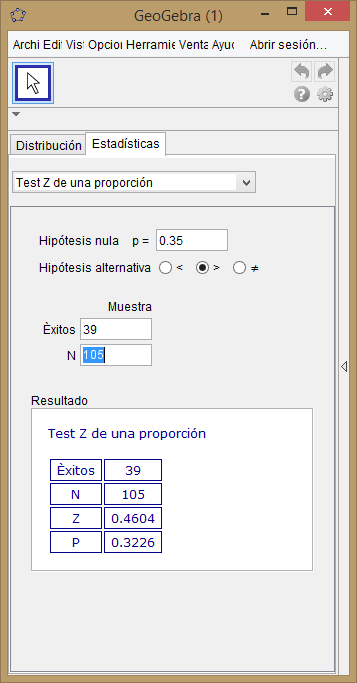
\includegraphics[width=7cm]{../fig/Tut08-09.png}\qquad
    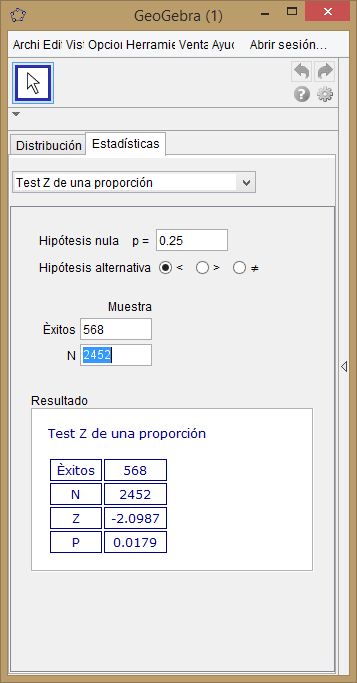
\includegraphics[width=7cm]{../fig/Tut08-10.png}
    \end{center}

\paragraph{\bf $\bullet$ Ejercicio \ref{tut08:ejercicio04}, pág. \pageref{tut08:ejercicio04}}
\label{tut08:ejercicio04:sol}\quad\\

\begin{enumerate}
  \item Con R sería
\begin{knitrout}
\definecolor{shadecolor}{rgb}{0.969, 0.969, 0.969}\color{fgcolor}\begin{kframe}
\begin{alltt}
\hlkwd{dpois}\hlstd{(}\hlnum{3}\hlstd{,} \hlkwc{lambda}\hlstd{=}\hlnum{2}\hlstd{)}
\end{alltt}
\begin{verbatim}
## [1] 0.18045
\end{verbatim}
\begin{alltt}
\hlkwd{dpois}\hlstd{(}\hlnum{10}\hlstd{,} \hlkwc{lambda}\hlstd{=}\hlnum{2}\hlstd{)}
\end{alltt}
\begin{verbatim}
## [1] 0.00003819
\end{verbatim}
\end{kframe}
\end{knitrout}

        En GeoGebra ejecutamos estos comandos:

        \begin{verbatim}
          Poisson[2, 3, false]

          Poisson[2, 10, false]
        \end{verbatim}
        Ten cuidado con el orden. En GeoGebra se coloca en primer lugar el valor de $\lambda$. Ten además en cuenta que si usas el panel de {\em Cálculo Simbólico} las respuestas serán (obviamente) simbólicas.

        En Wolfram Alpha usaríamos los comandos:
        \begin{verbatim}
          P(X=3) for X~Poisson(2)

          P(X=10) for X~Poisson(2)
        \end{verbatim}

  \item El cálculo con R es:
\begin{knitrout}
\definecolor{shadecolor}{rgb}{0.969, 0.969, 0.969}\color{fgcolor}\begin{kframe}
\begin{alltt}
\hlkwd{ppois}\hlstd{(}\hlnum{2400}\hlstd{,} \hlkwc{lambda}\hlstd{=}\hlnum{2489}\hlstd{)}
\end{alltt}
\begin{verbatim}
## [1] 0.037438
\end{verbatim}
\end{kframe}
\end{knitrout}
        Con GeoGebra el comando es:
        \begin{verbatim}
          Poisson[2489, 2400, true]
        \end{verbatim}
        La respuesta simbólica (al cabo de unos segundos) es excesivamente larga como para incluirla aquí. De hecho, en la versión 5.0.44  para Windows de GeoGebra este calculo simbólico  funciona, pero produce un error en la versión 5.0.24 para Mac OSX.

        Puedes ver la respuesta simbólica completa más fácilmente usando este comando en Wolfram Alpha:
        \begin{verbatim}
        P(X<=2489) for X~Poisson(2400)
        \end{verbatim}



\end{enumerate}



\paragraph{\bf $\bullet$ Ejercicio \ref{tut08:ejercicio05}, pág. \pageref{tut08:ejercicio05}}
\label{tut08:ejercicio05:sol}\quad\\

El comando necesario en Wolfram Alpha es:
\begin{verbatim}
  sum((k - lambda)^2 * exp(-lambda) *  lambda^k / k!) from k=0 to oo
\end{verbatim}


%#########################################################################################
%#########################################################################################
\vspace{2cm} \hrule
\quad\\
Fin del Tutorial08. ¡Gracias por la atención!


%\newpage
%\addcontentsline{toc}{section}{Guía de trabajo.}
%\includepdf[pages={1-},scale=0.90]{08-GuiaDeTrabajo.pdf}


\end{document}



